\section{Bằng chứng bảo mật}
\label{sec:security}

Phần này cung cấp bằng chứng chi tiết về các biện pháp bảo mật đã được triển khai trong hệ thống, bao gồm screenshots và giải thích cho từng yêu cầu bảo mật.

\subsection{Frontend Security Evidence}
\label{ssec:frontend_security}

\subsubsection{SE-1: S3 Block Public Access Enabled}

Hình \ref{fig:se1} cho thấy S3 bucket đã được cấu hình với tất cả 4 Block Public Access options được bật. Điều này đảm bảo bucket hoàn toàn private và không thể truy cập trực tiếp từ Internet.

\begin{figure}[H]
\centering
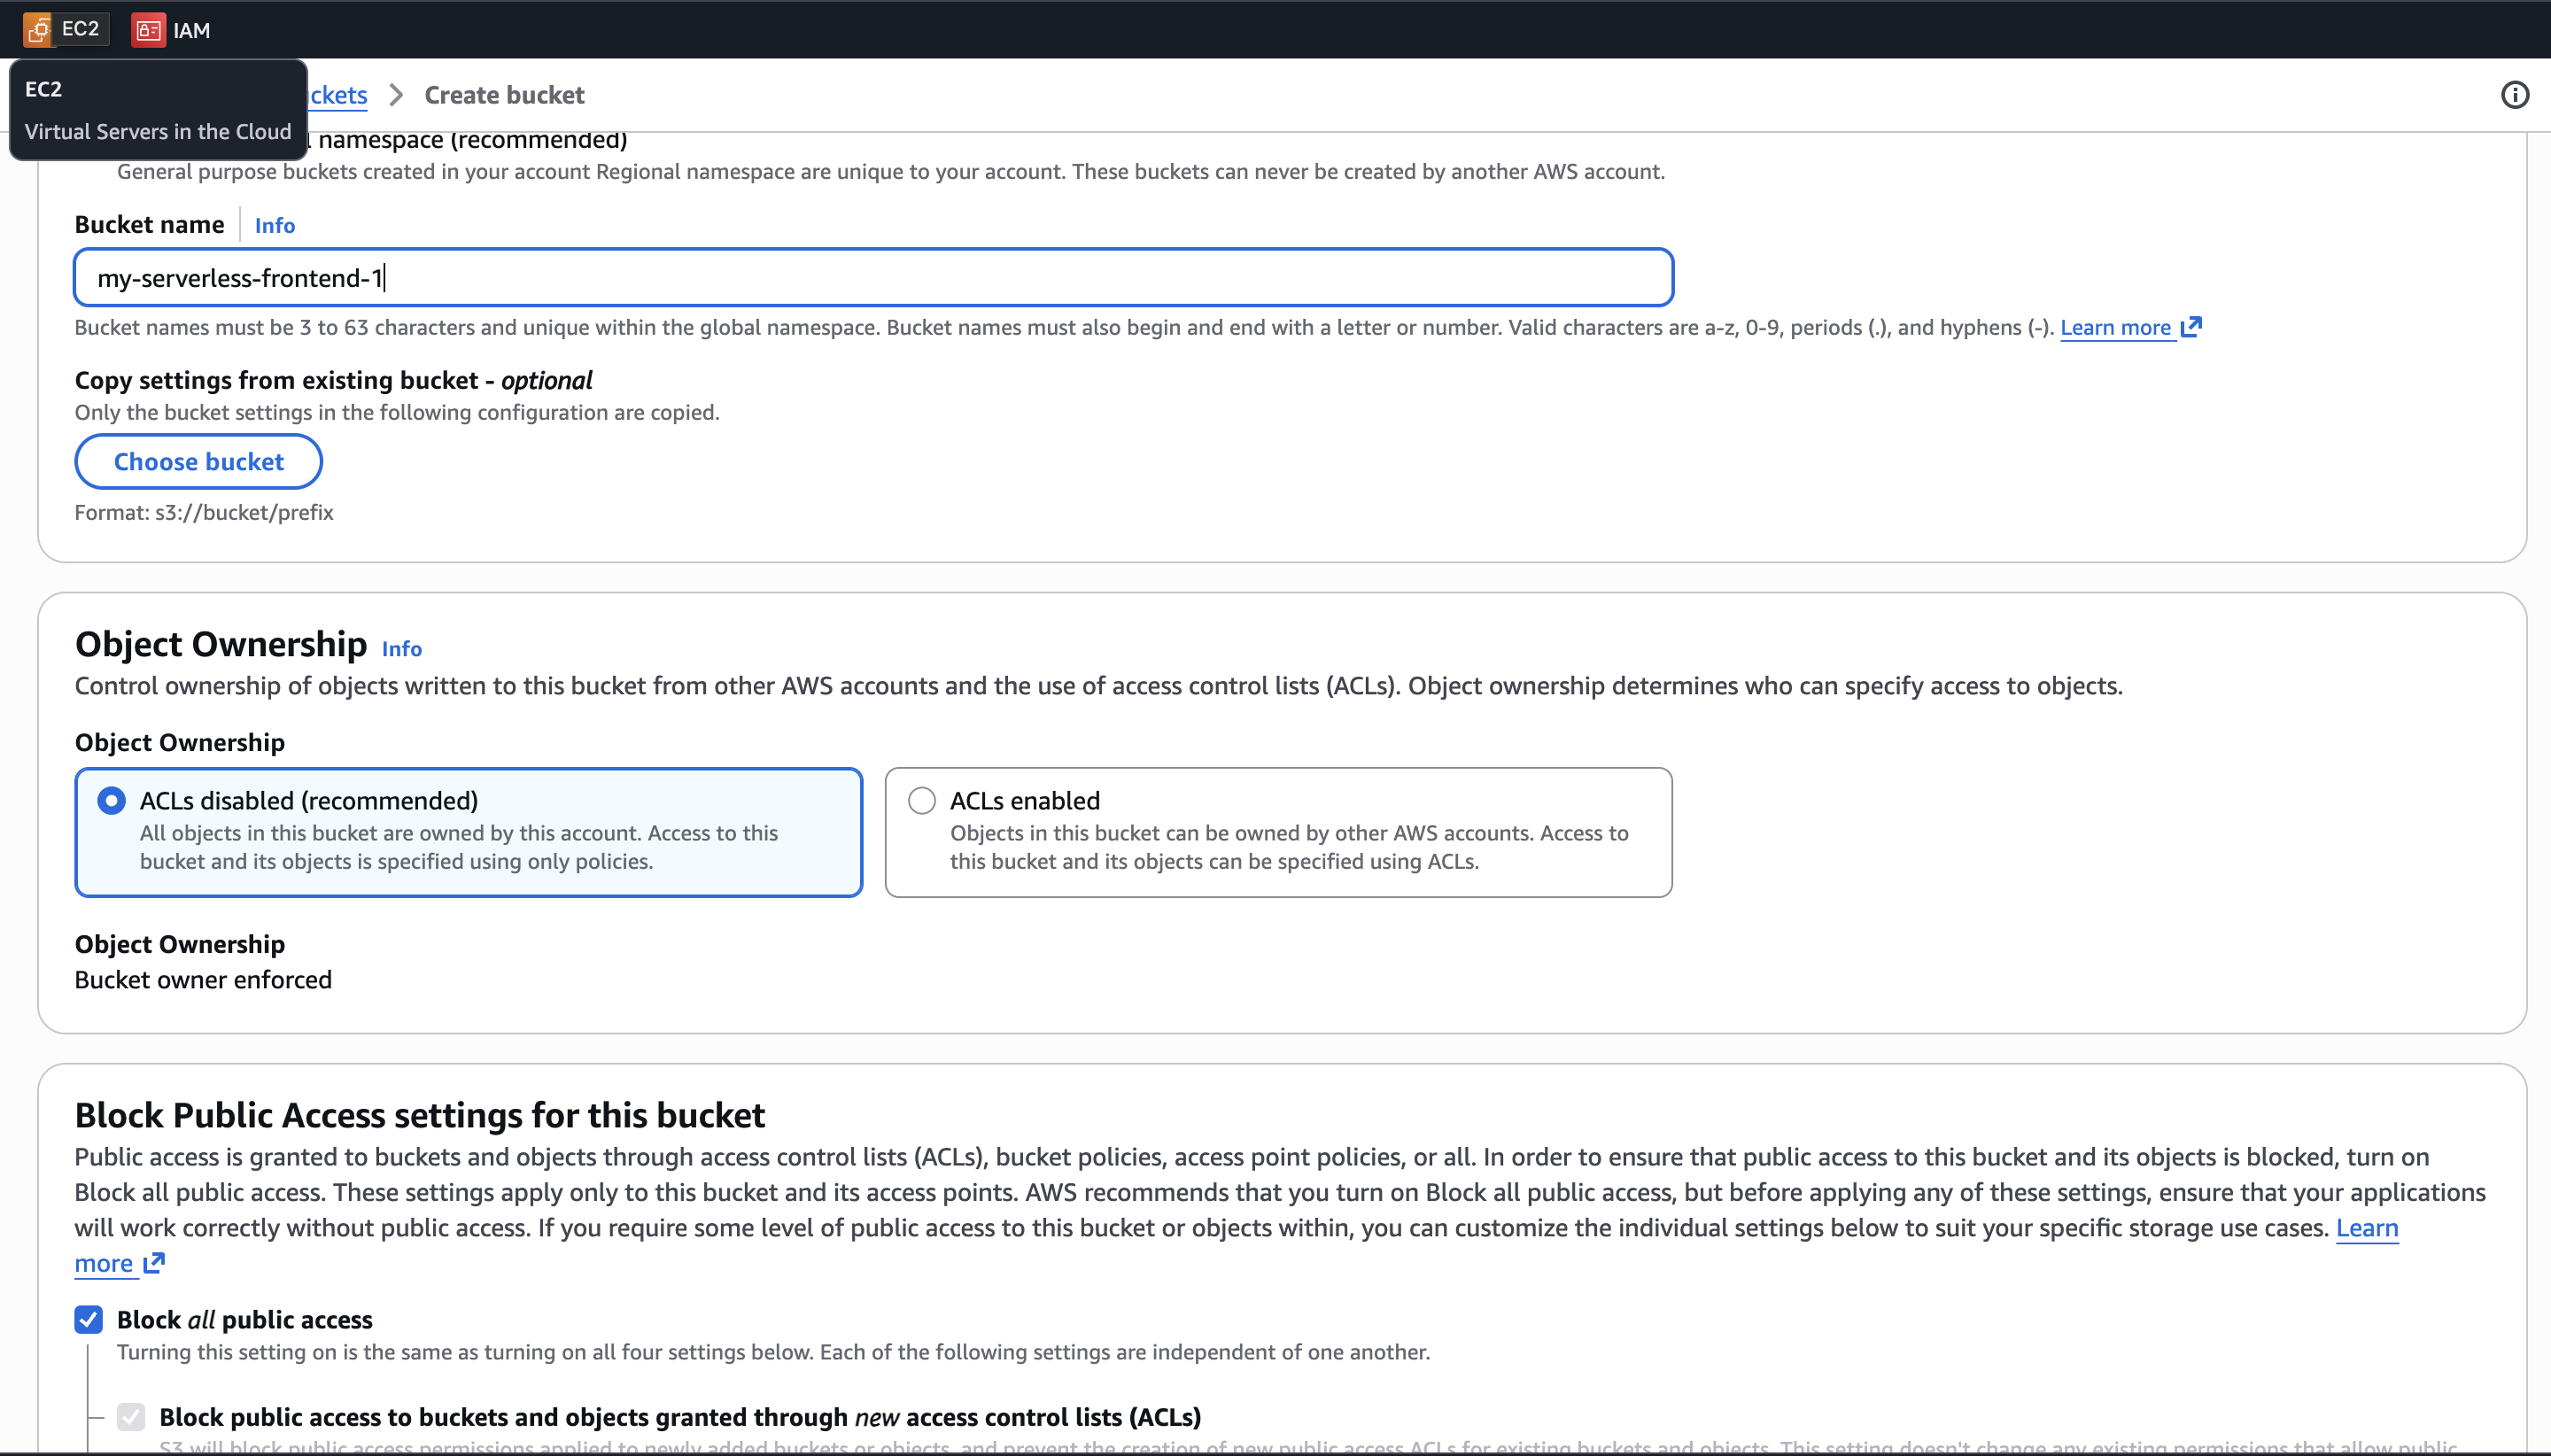
\includegraphics[width=0.9\textwidth]{img/SE-1_s3_block_public_access.png}
\caption{S3 Block Public Access - Tất cả 4 options được bật}
\label{fig:se1}
\end{figure}

Các options được bật:
\begin{itemize}
    \item Block all public access
    \item Block public access to buckets and objects granted through new ACLs
    \item Block public access to buckets and objects granted through any ACLs
    \item Block public access to buckets and objects granted through new public bucket or access point policies
\end{itemize}

\subsubsection{SE-2: Direct S3 Access Rejected}

Hình \ref{fig:se2} minh chứng rằng khi truy cập trực tiếp vào S3 URL, request bị từ chối với mã lỗi 403 Forbidden. Điều này xác nhận bucket không thể truy cập công khai.

\begin{figure}[H]
\centering
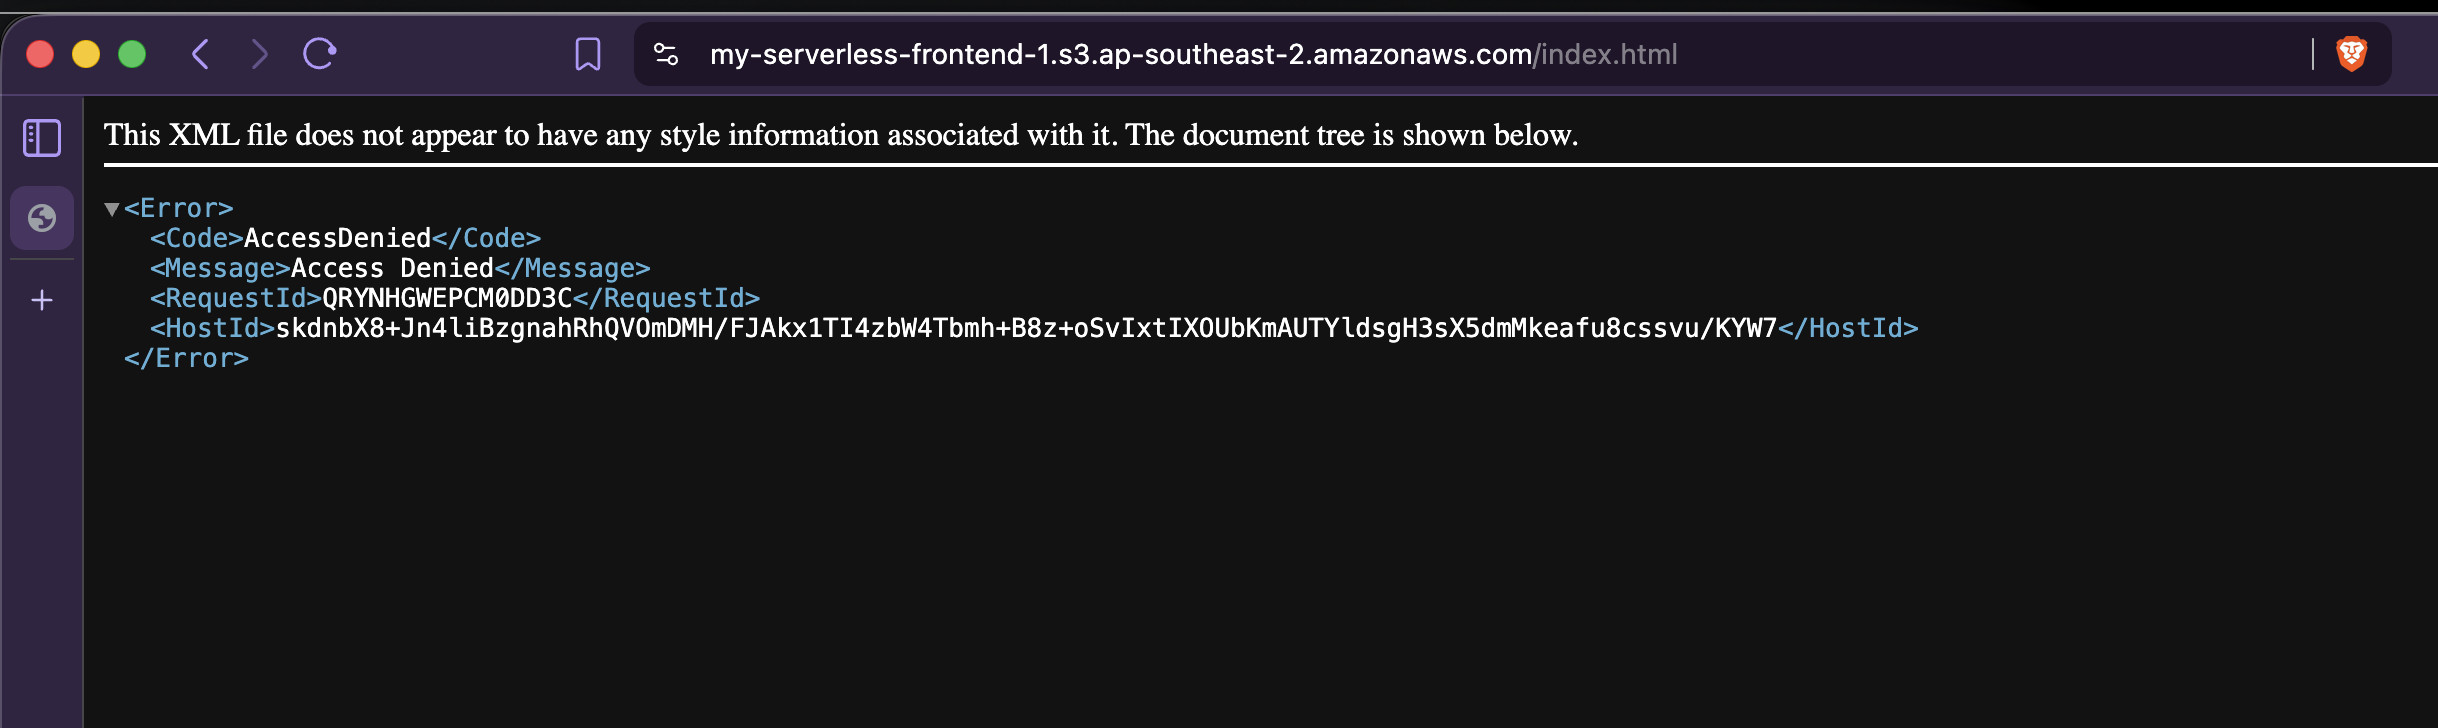
\includegraphics[width=0.9\textwidth]{img/SE-2_s3_403_forbidden.png}
\caption{Truy cập trực tiếp S3 URL bị từ chối với 403 Forbidden}
\label{fig:se2}
\end{figure}

Test command đã thực hiện:
\begin{verbatim}
curl https://bucket-name.s3.ap-southeast-1.amazonaws.com/index.html
\end{verbatim}

Kết quả: Access Denied - xác nhận S3 bucket đã được bảo vệ đúng cách.

\subsubsection{SE-3: CloudFront Access Succeeds}

Hình \ref{fig:se3} cho thấy khi truy cập qua CloudFront URL, ứng dụng hoạt động bình thường với status code 200 OK. Điều này chứng minh CloudFront có thể đọc từ S3 thông qua OAC.

\begin{figure}[H]
\centering
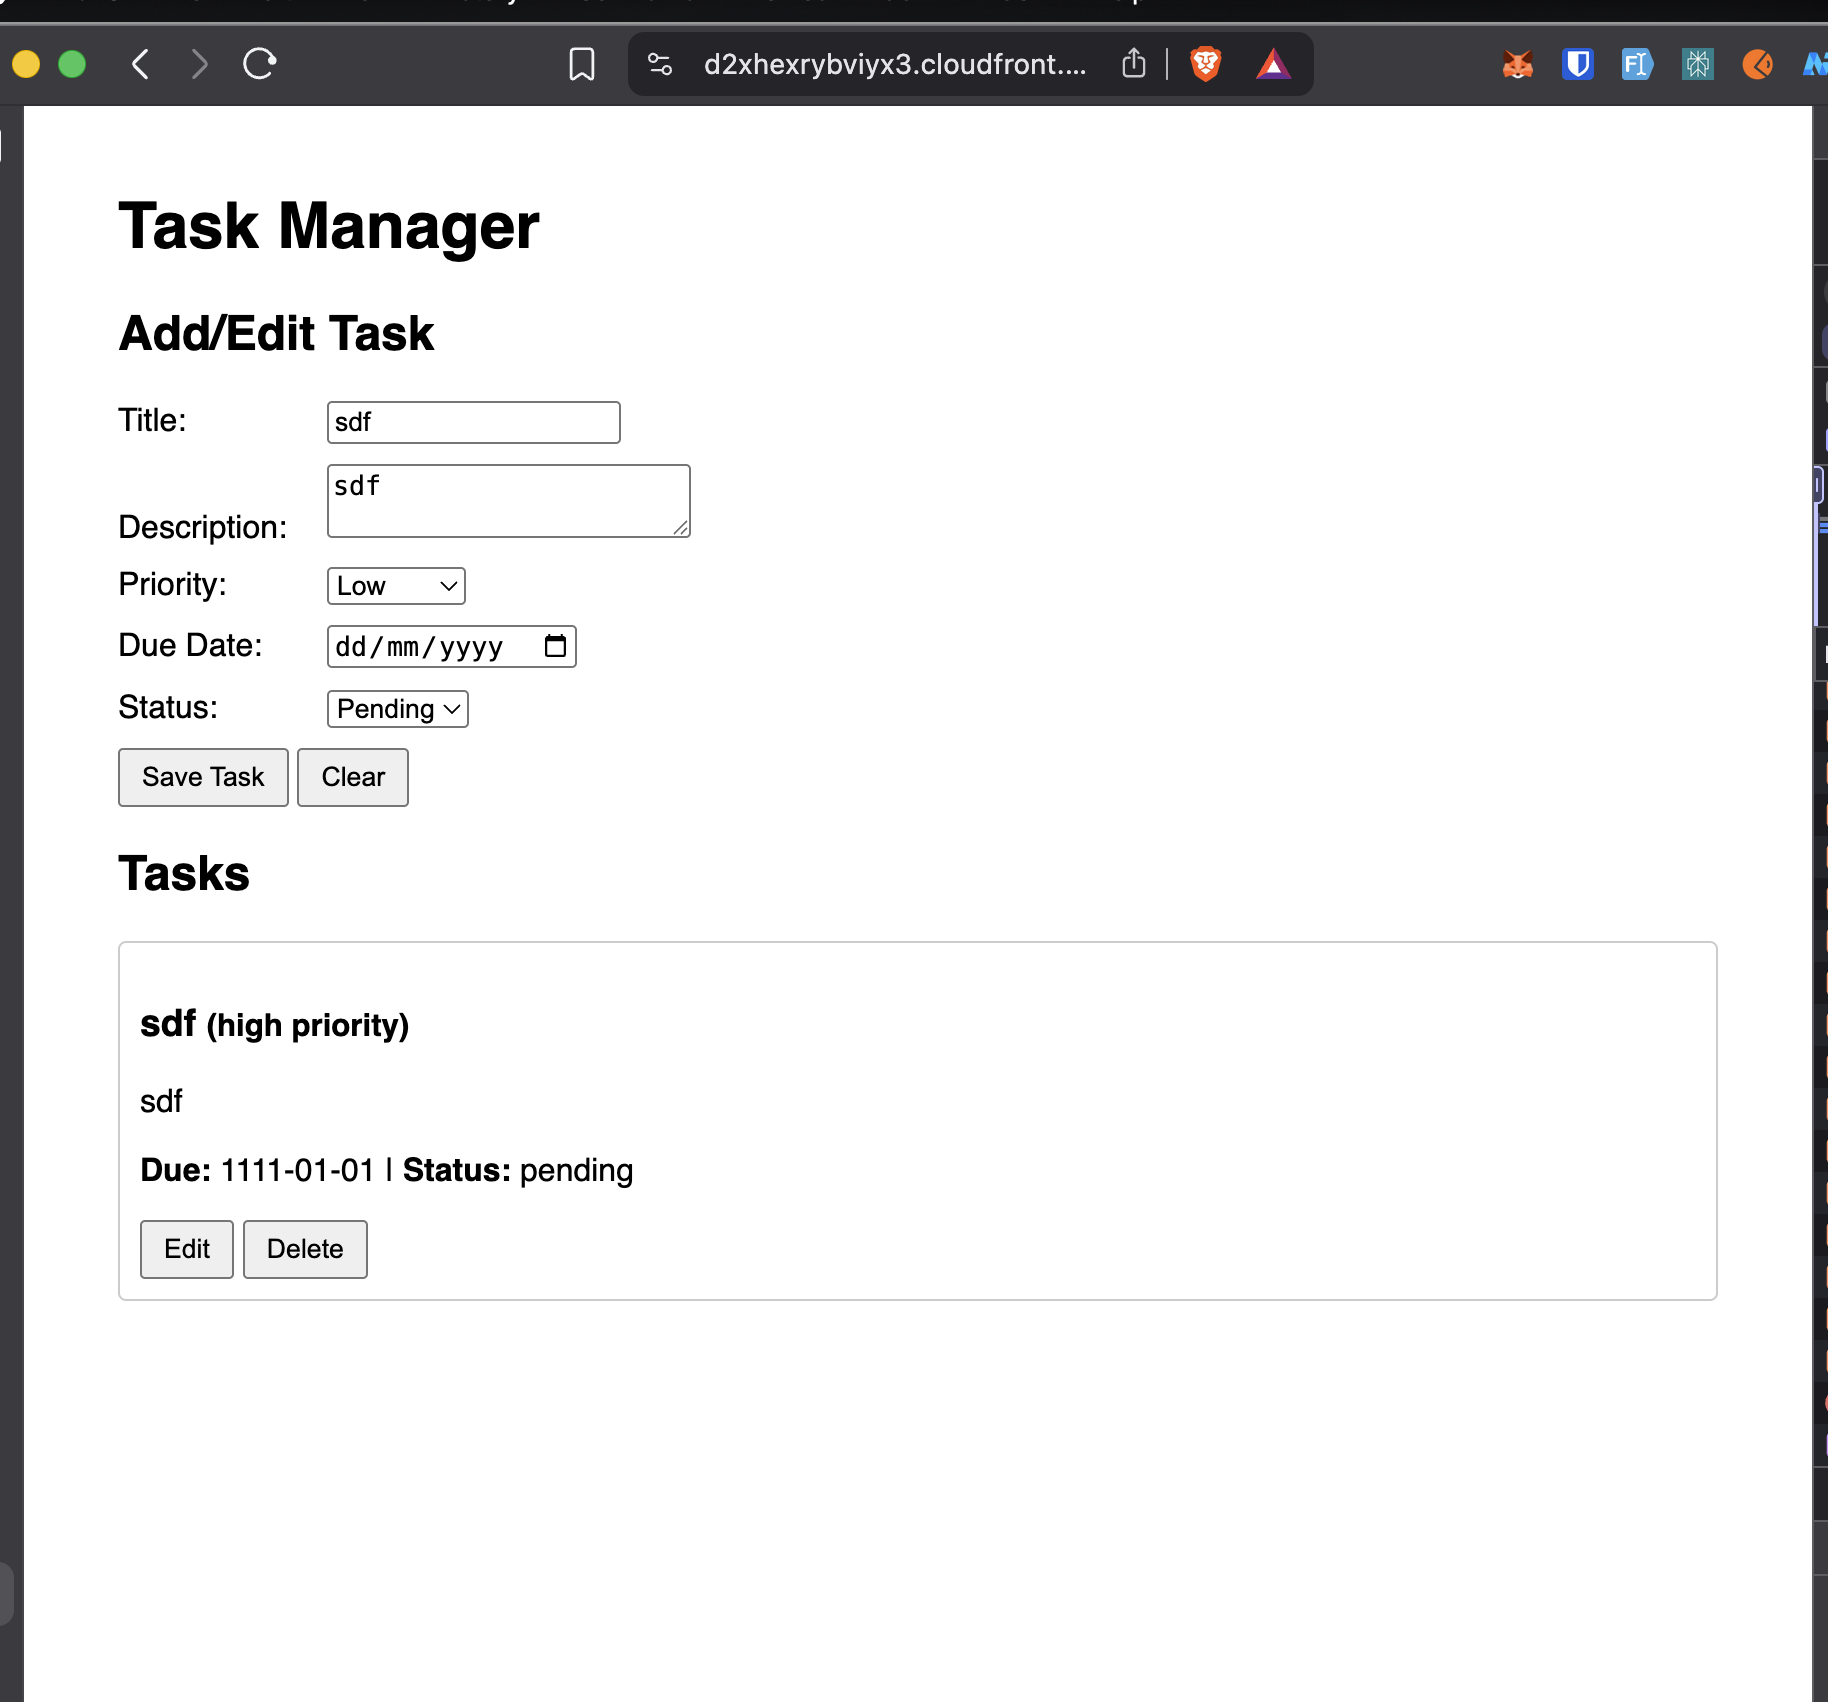
\includegraphics[width=0.9\textwidth]{img/SE-3_cloudfront_200.png}
\caption{Truy cập qua CloudFront URL thành công với 200 OK}
\label{fig:se3}
\end{figure}

CloudFront URL: https://d1234567.cloudfront.net

\subsubsection{SE-4: OAC Attached to CloudFront}

Hình \ref{fig:se4a} và \ref{fig:se4b} hiển thị cấu hình CloudFront distribution với Origin Access Control (OAC) được attach. OAC cho phép CloudFront đọc từ S3 private bucket một cách an toàn.

\begin{figure}[H]
\centering
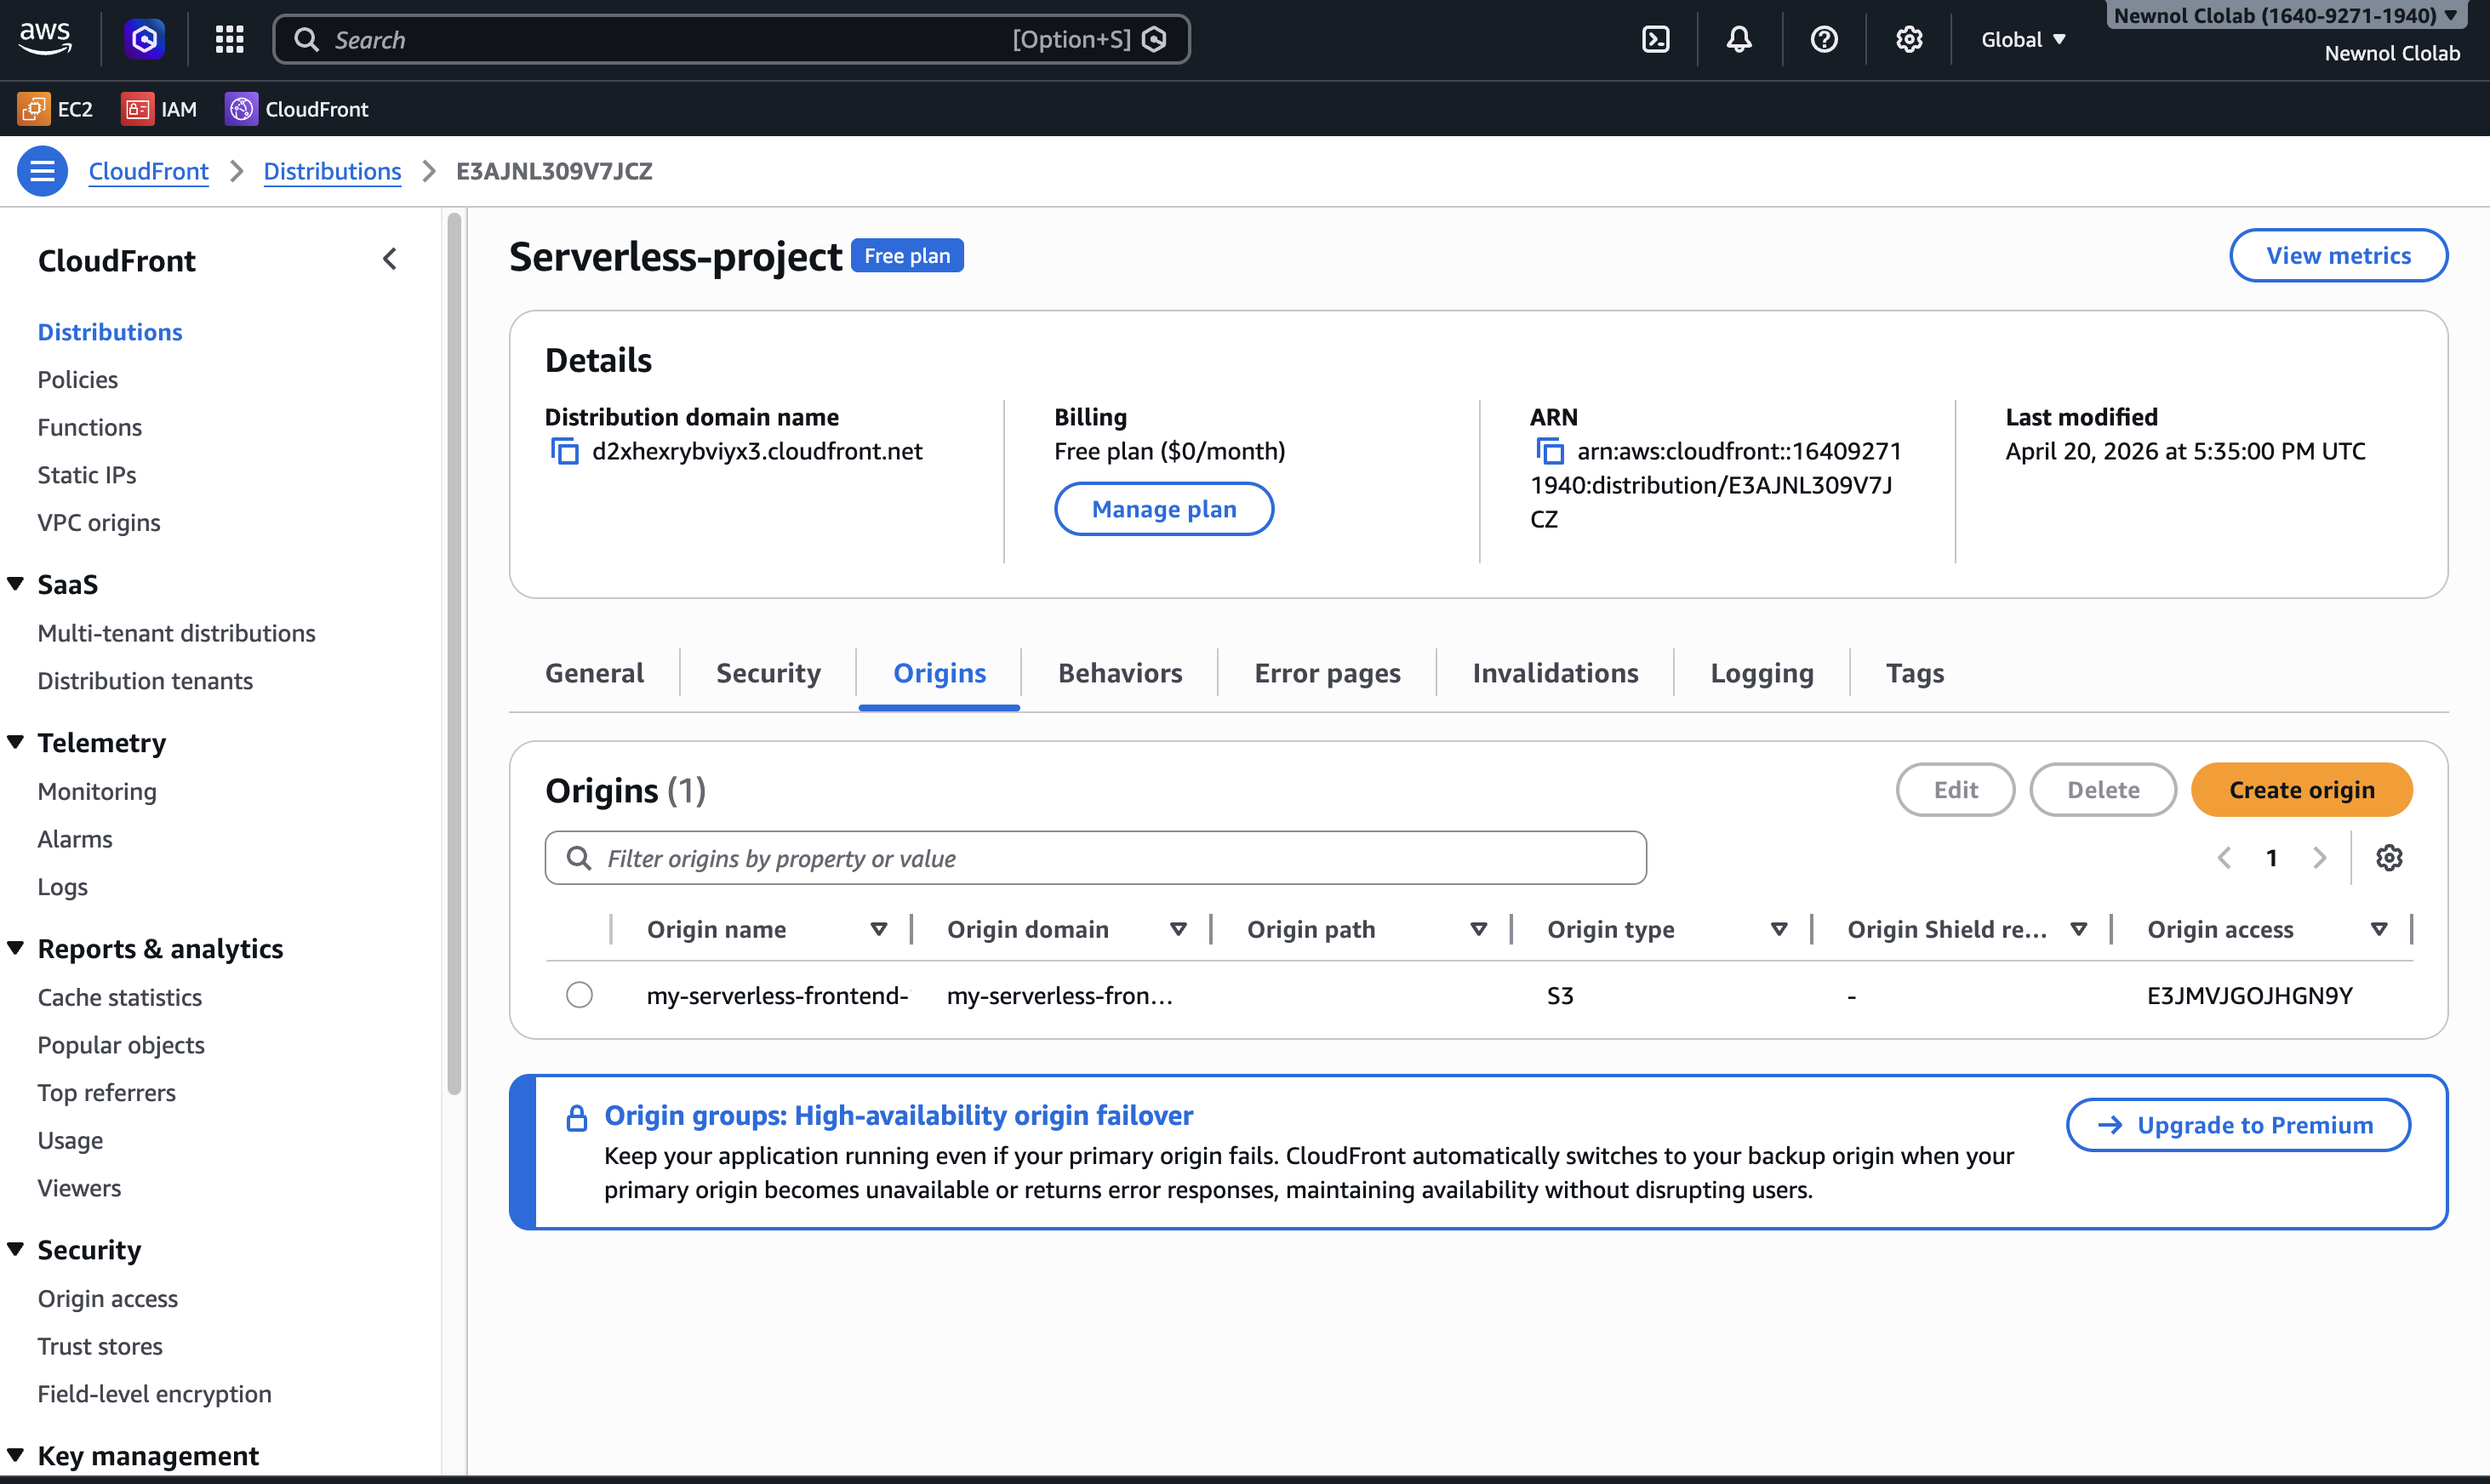
\includegraphics[width=0.9\textwidth]{img/SE-4_cloudfront_oac_1.png}
\caption{CloudFront Origin settings với OAC}
\label{fig:se4a}
\end{figure}

\begin{figure}[H]
\centering
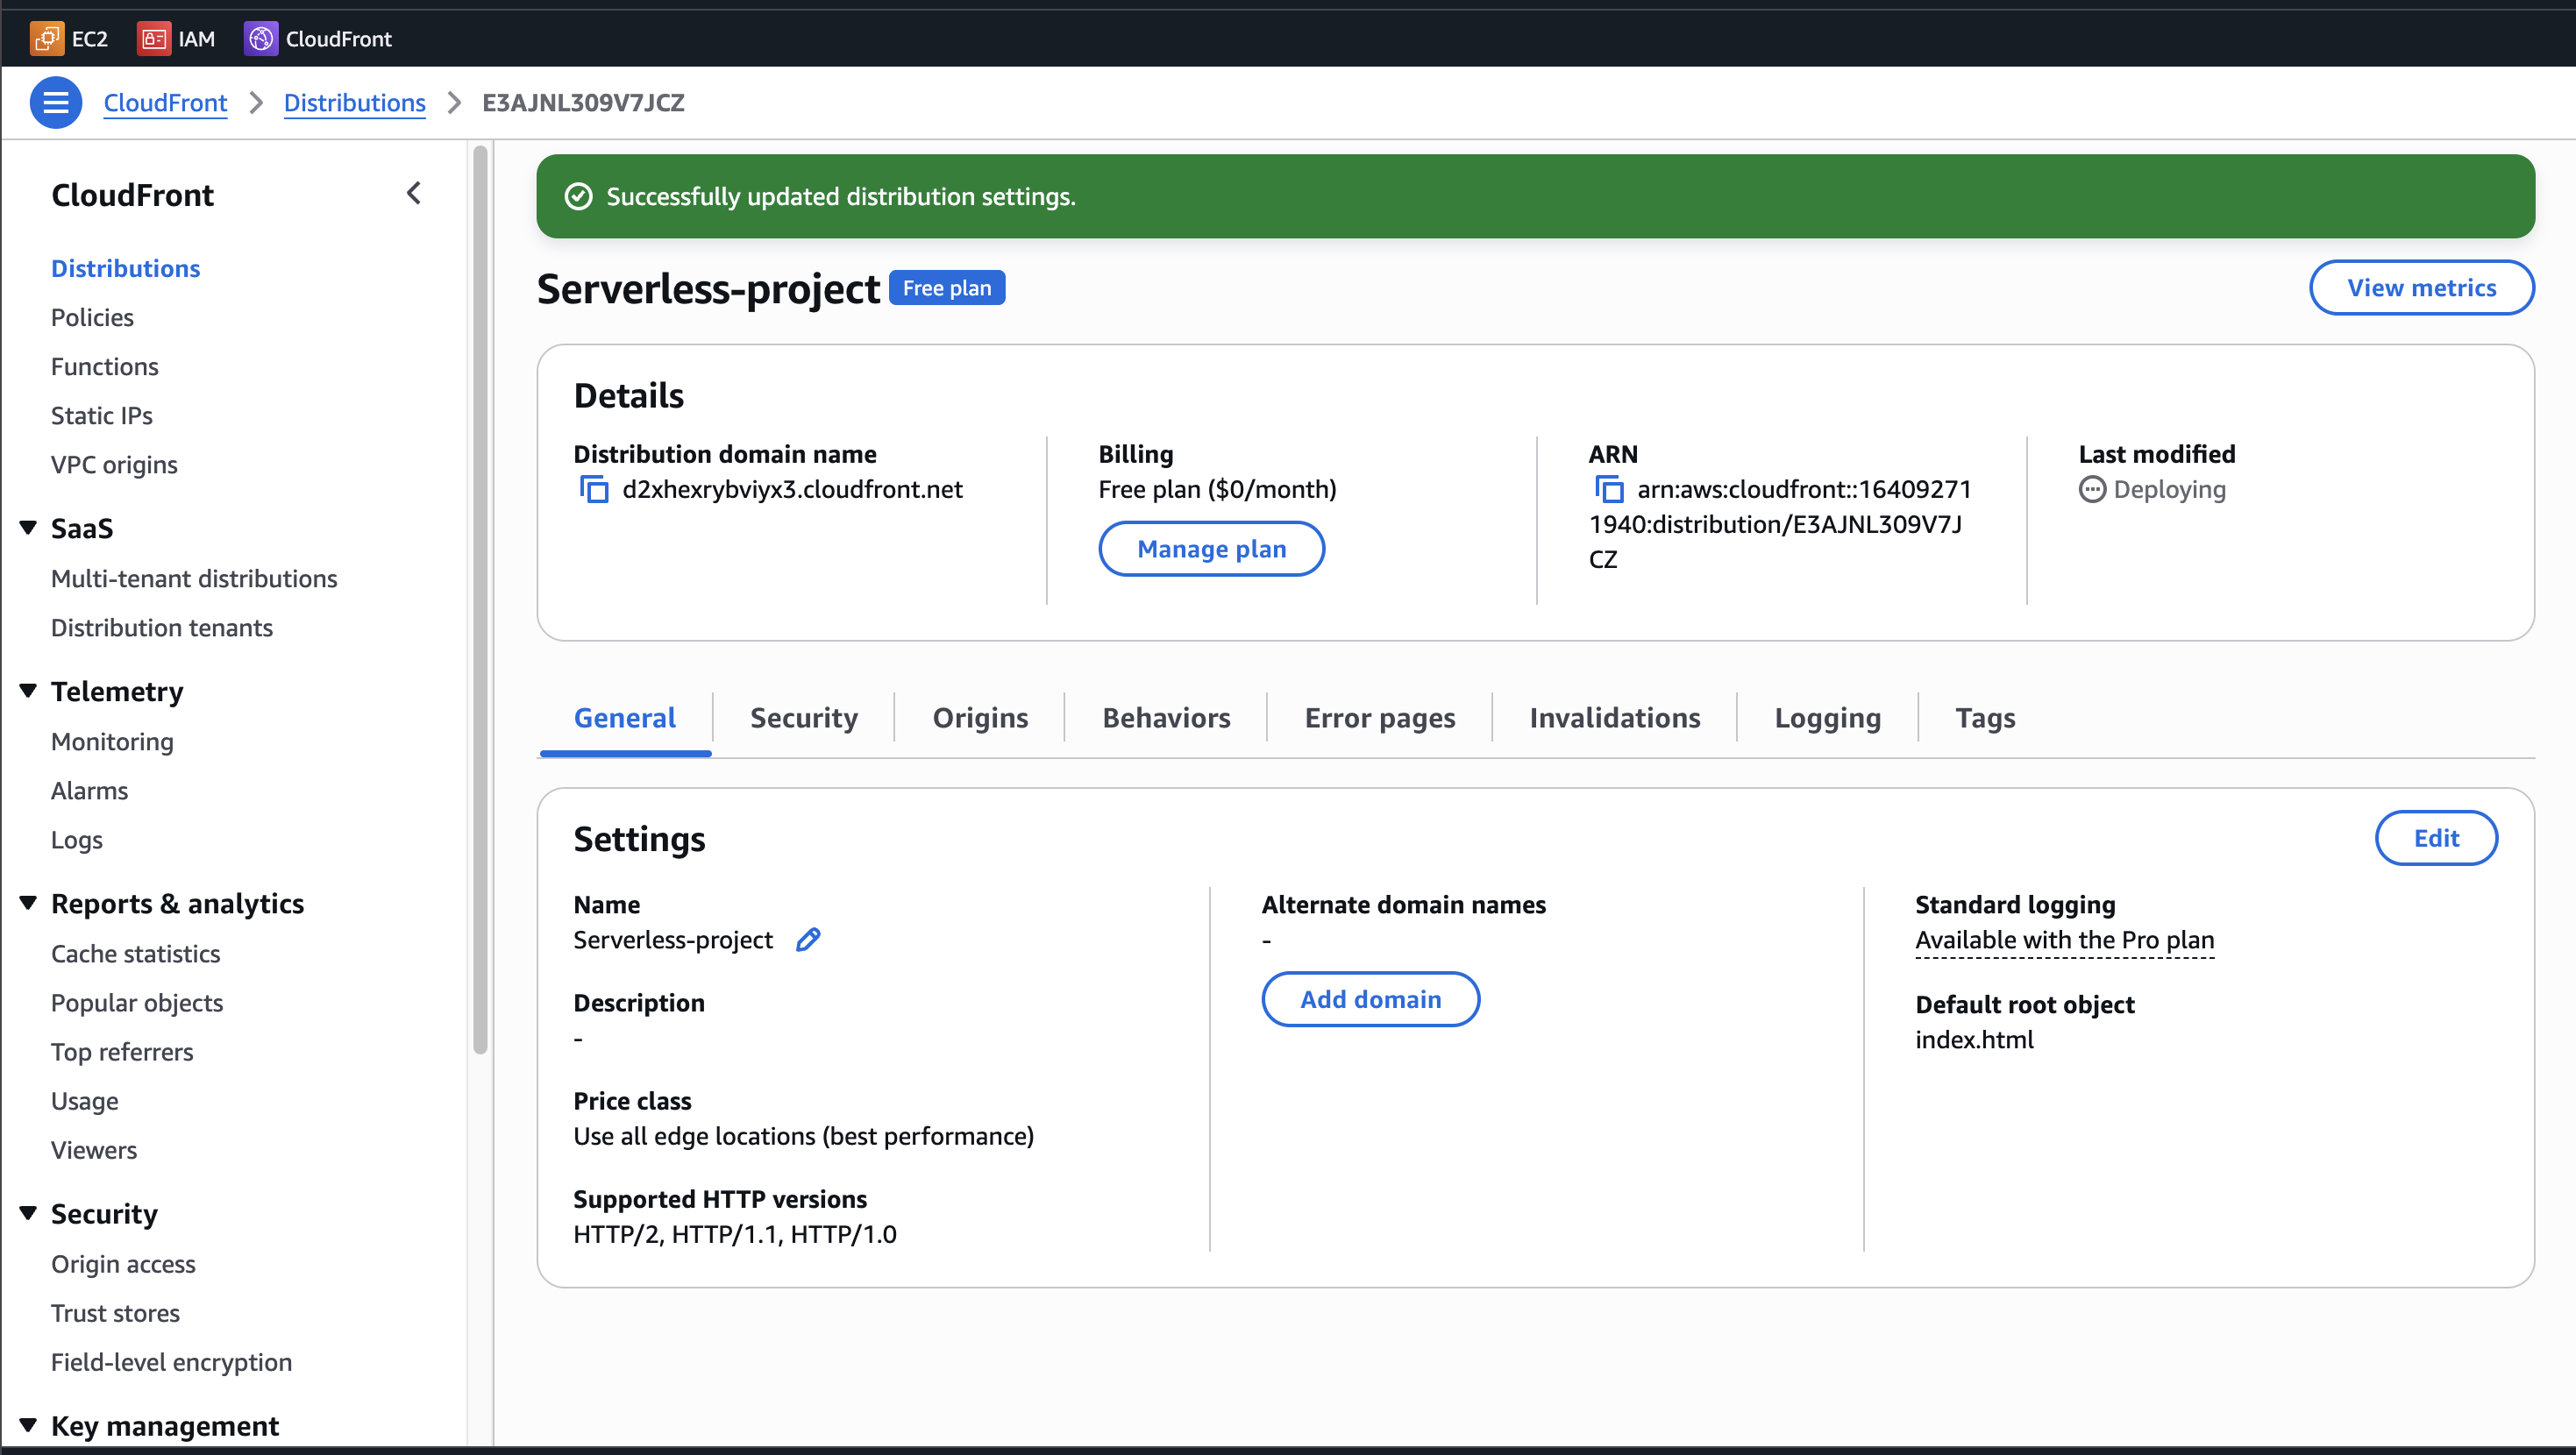
\includegraphics[width=0.9\textwidth]{img/SE-4_cloudfront_oac_2.png}
\caption{Chi tiết OAC configuration}
\label{fig:se4b}
\end{figure}

Origin Access Control settings:
\begin{itemize}
    \item Origin access: Origin access control settings (recommended)
    \item OAC name: task-manager-oac
    \item Signing behavior: Sign requests (recommended)
    \item Origin type: S3
\end{itemize}

\subsection{Networking Security Evidence}
\label{ssec:network_security}

\subsubsection{NE-1: VPC Endpoint Created for DynamoDB}

Hình \ref{fig:ne1} cho thấy VPC Gateway Endpoint cho DynamoDB đã được tạo thành công với status Available. Endpoint này cho phép Lambda kết nối DynamoDB qua mạng private của AWS.

\begin{figure}[H]
\centering
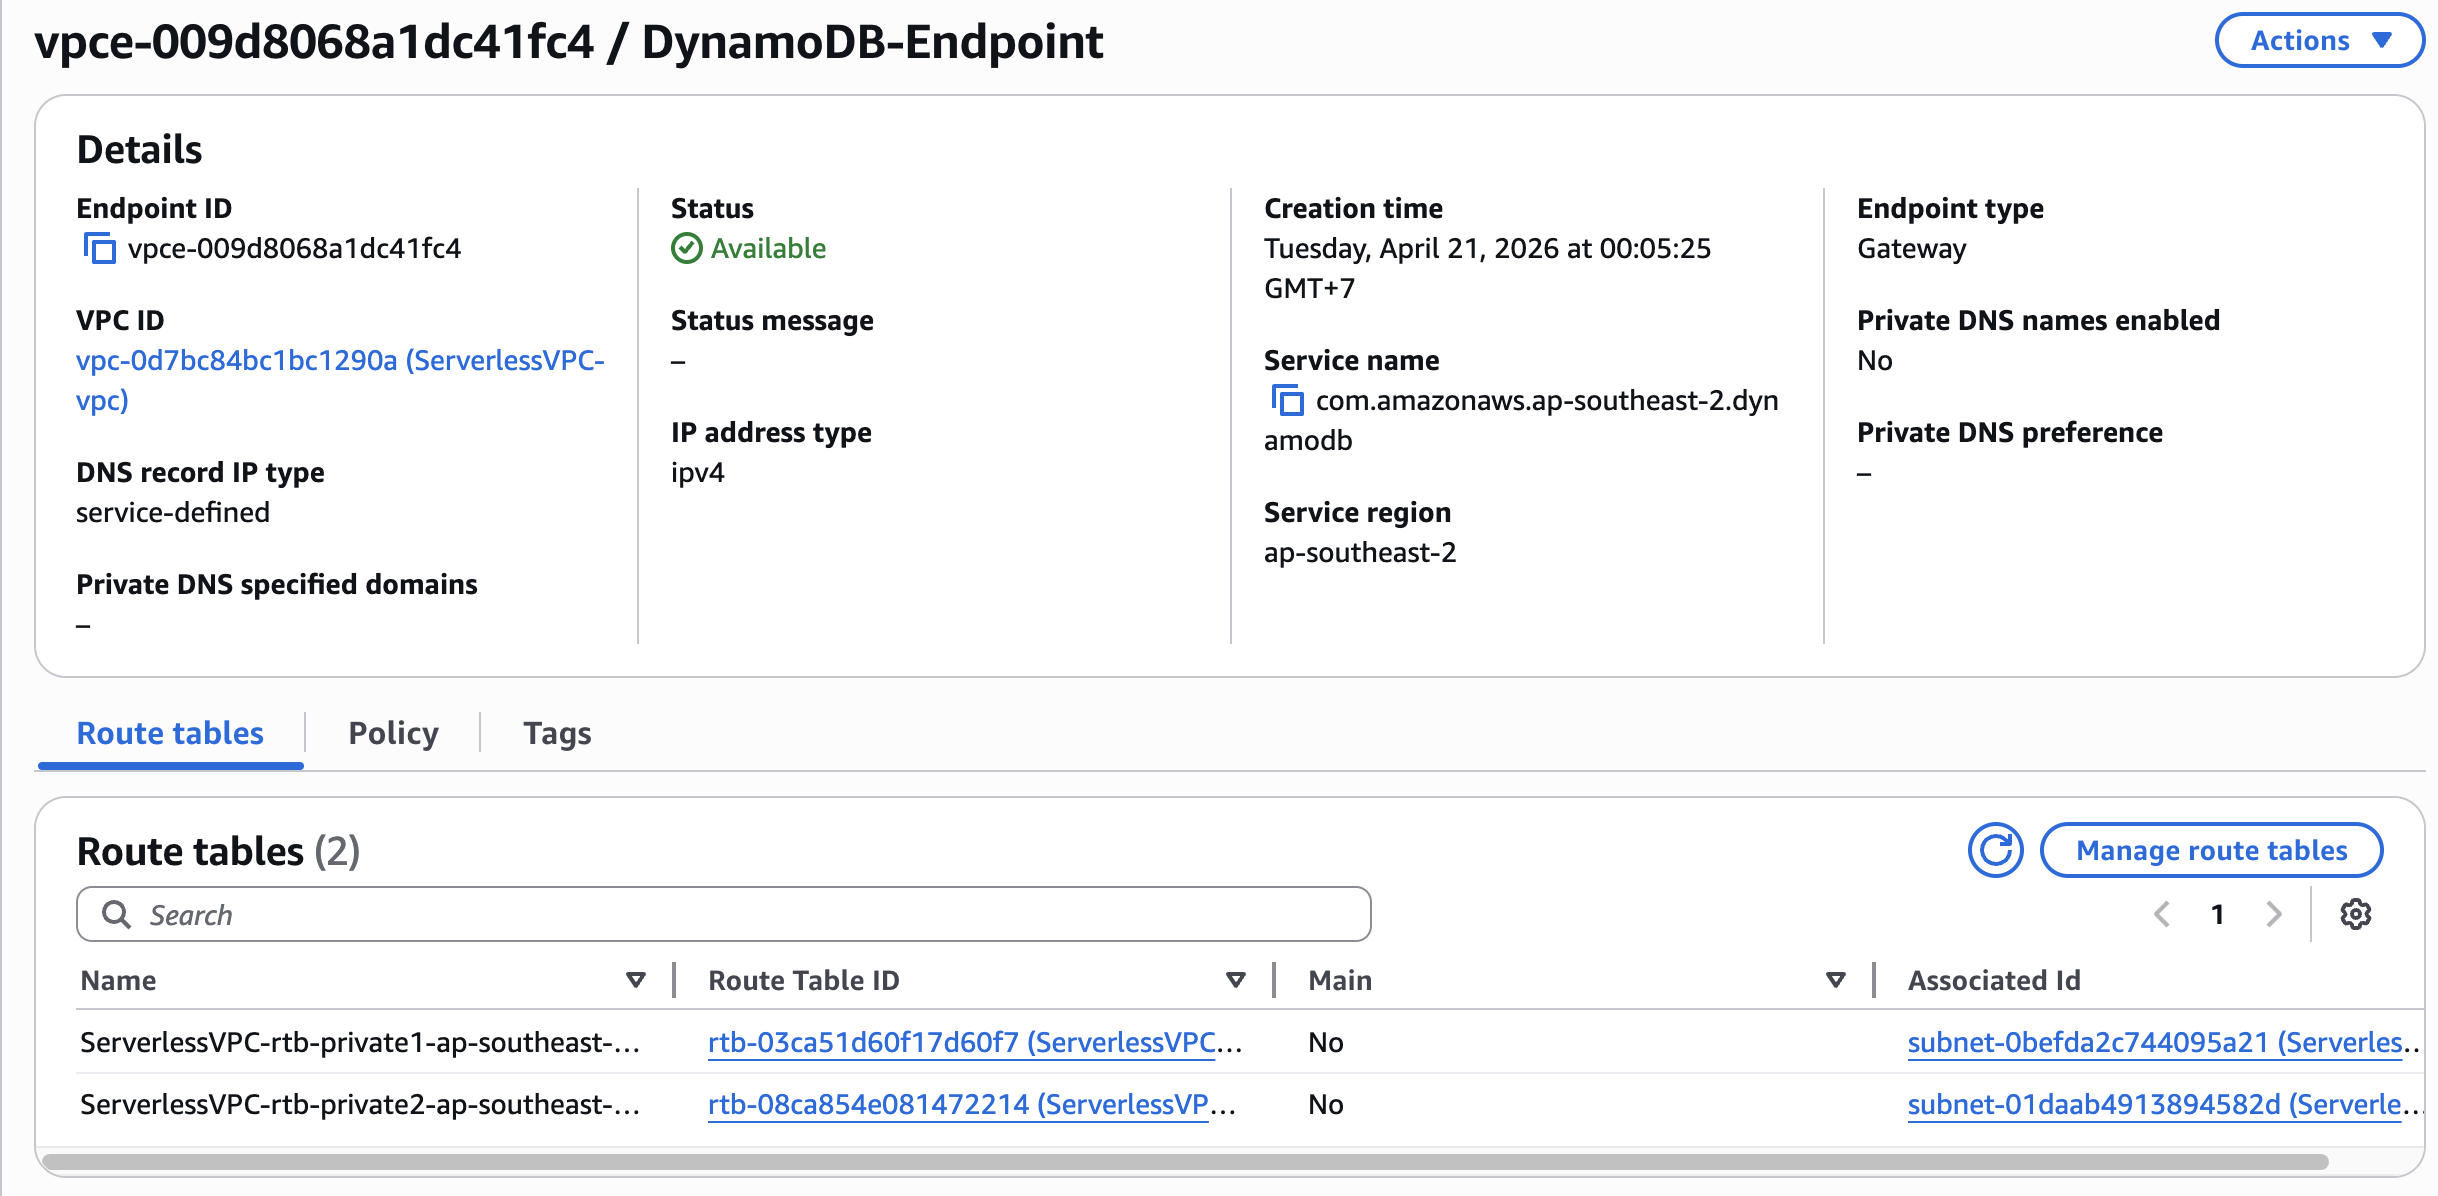
\includegraphics[width=0.9\textwidth]{img/NE-1_vpc_endpoint.png}
\caption{VPC Gateway Endpoint cho DynamoDB với status Available}
\label{fig:ne1}
\end{figure}

Thông tin endpoint:
\begin{itemize}
    \item Service name: com.amazonaws.ap-southeast-1.dynamodb
    \item Type: Gateway
    \item Status: Available
    \item VPC: Custom VPC (10.0.0.0/16)
    \item Route tables: Private Route Table
\end{itemize}

\subsubsection{NE-2: Lambda Has VpcConfig}

Hình \ref{fig:ne2} minh chứng Lambda function đã được attach vào VPC với cấu hình VpcConfig bao gồm subnets và security group.

\begin{figure}[H]
\centering
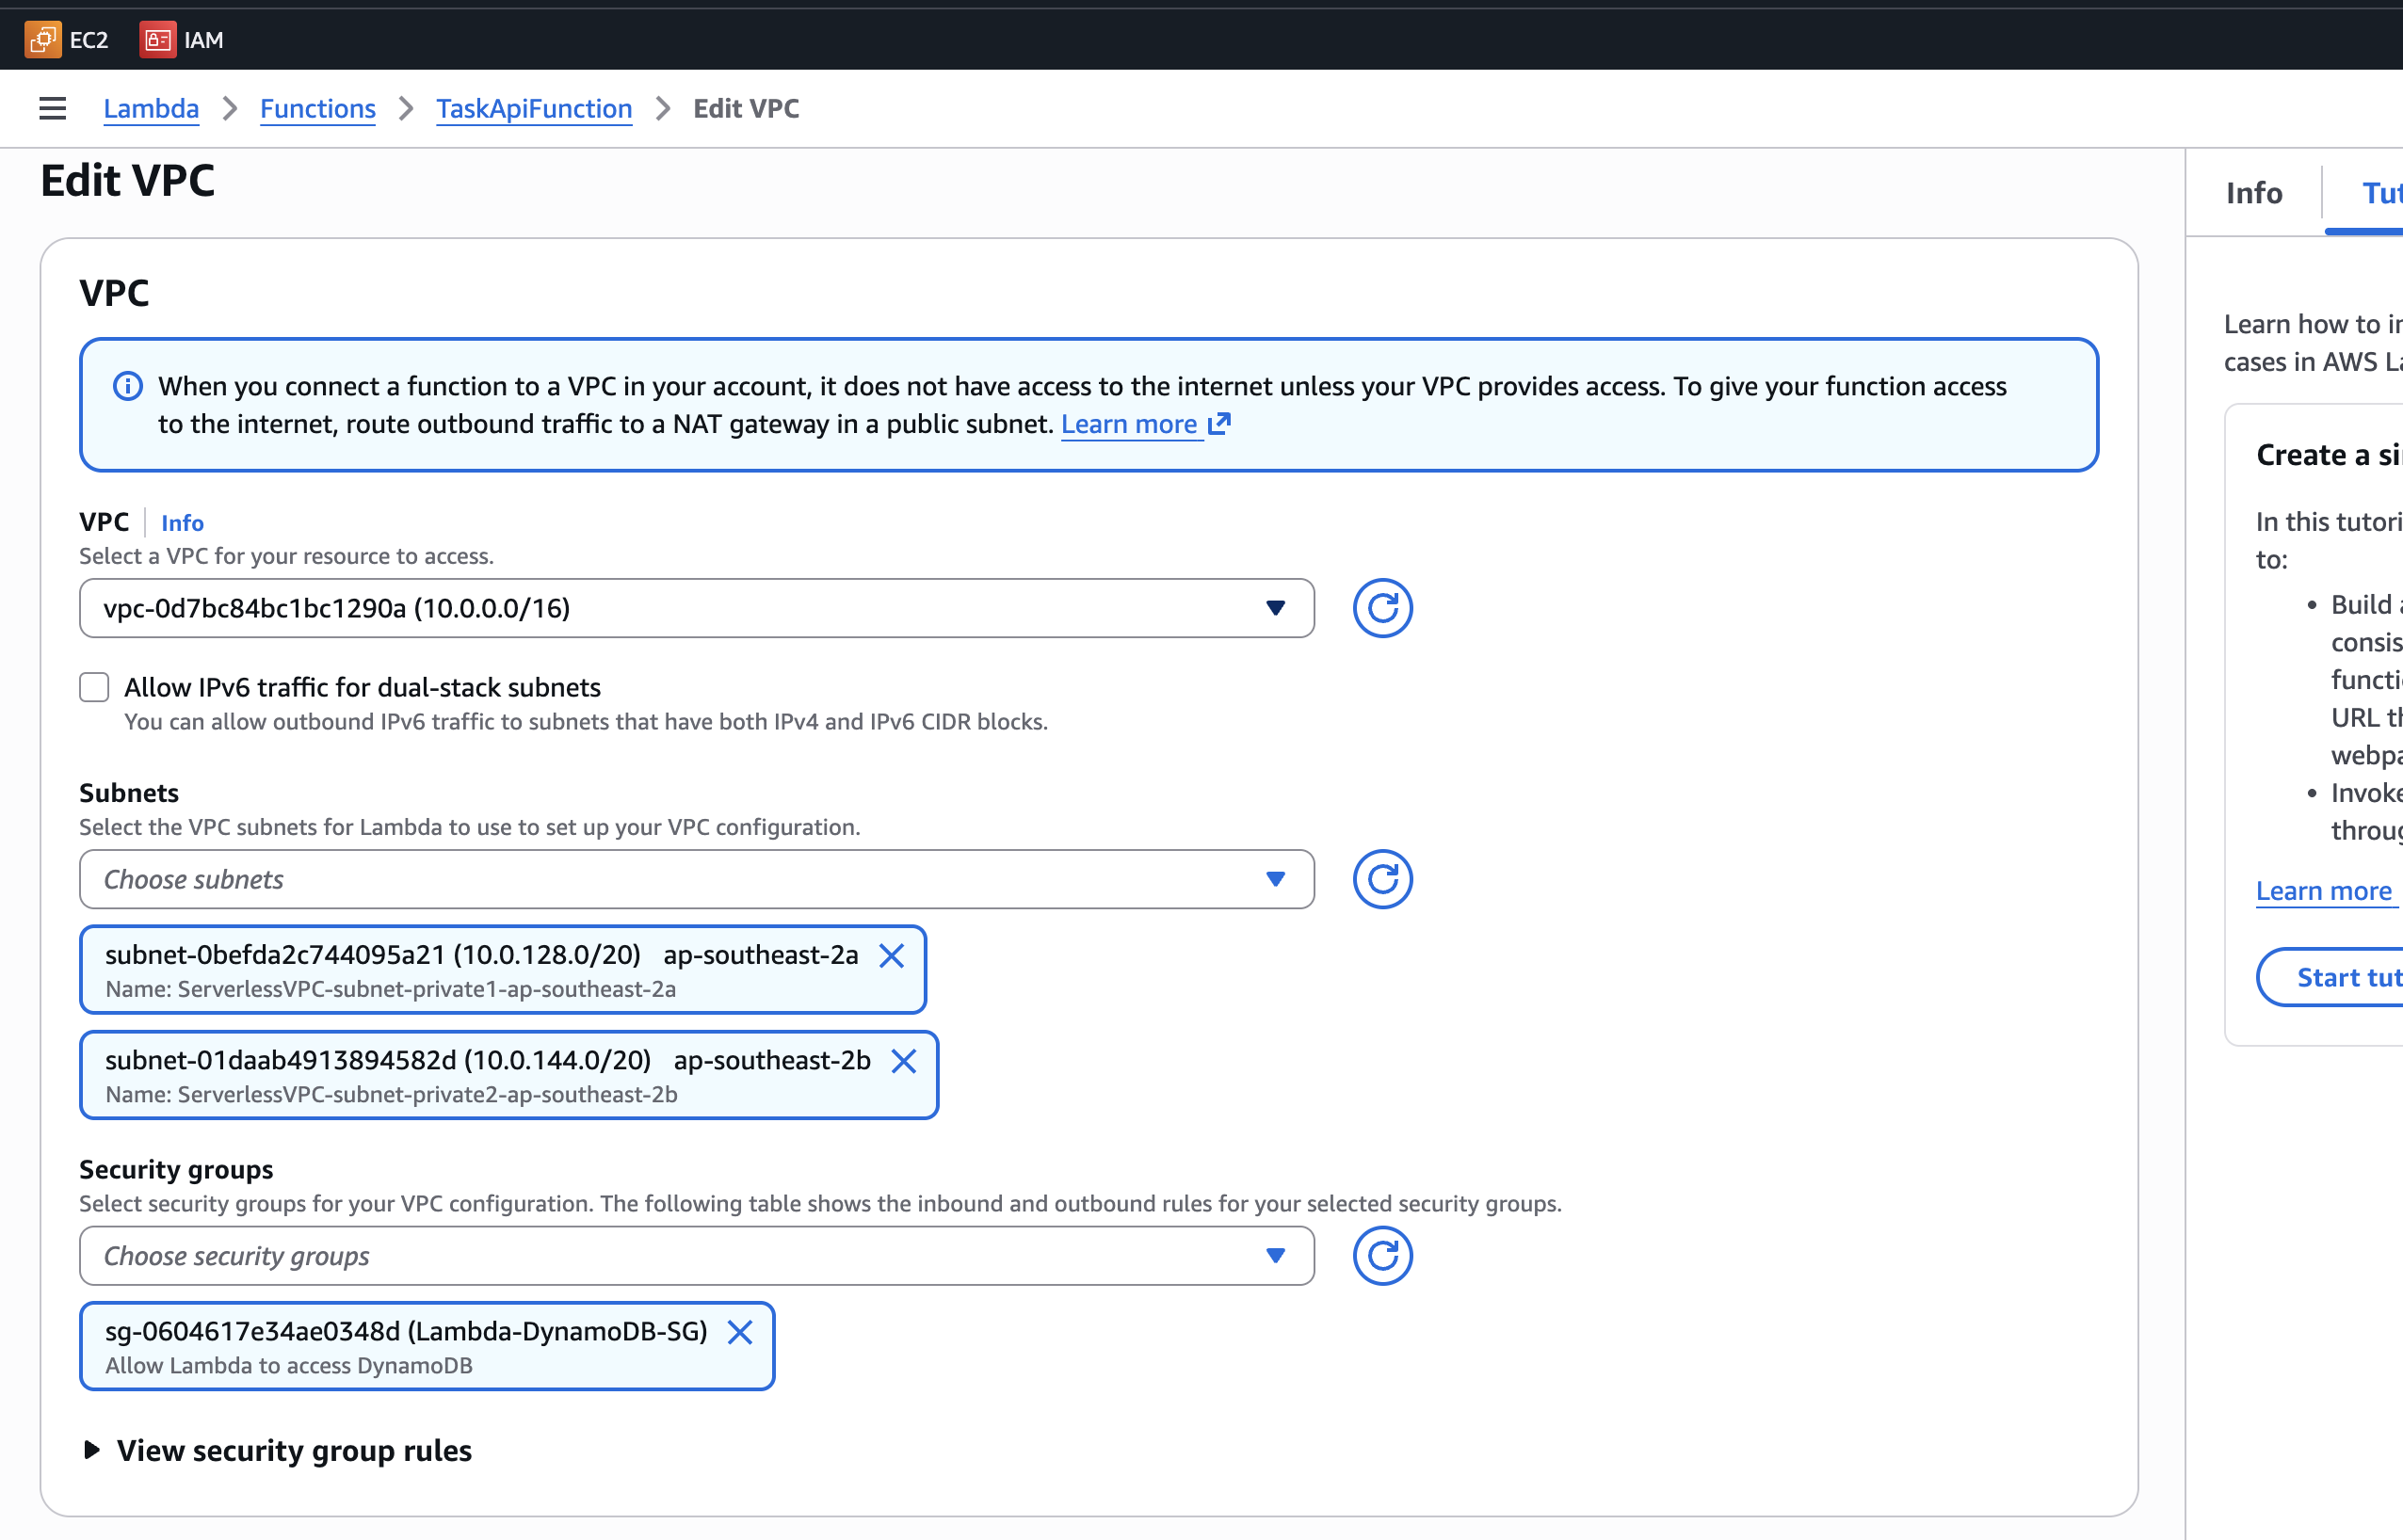
\includegraphics[width=0.9\textwidth]{img/NE-2_lambda_vpc_config.png}
\caption{Lambda VPC Configuration với subnets và security group}
\label{fig:ne2}
\end{figure}

VPC Configuration:
\begin{itemize}
    \item VPC: Custom VPC
    \item Subnets: Private Subnet A (10.0.1.0/24), Private Subnet B (10.0.2.0/24)
    \item Security groups: lambda-sg
    \item Network interfaces: ENI được tạo tự động trong các subnets
\end{itemize}

\subsubsection{NE-3: Route Table Has Endpoint Route}

Hình \ref{fig:ne3} hiển thị Private Route Table với route entry trỏ đến VPC Endpoint. Route này đảm bảo traffic đến DynamoDB đi qua endpoint thay vì Internet.

\begin{figure}[H]
\centering
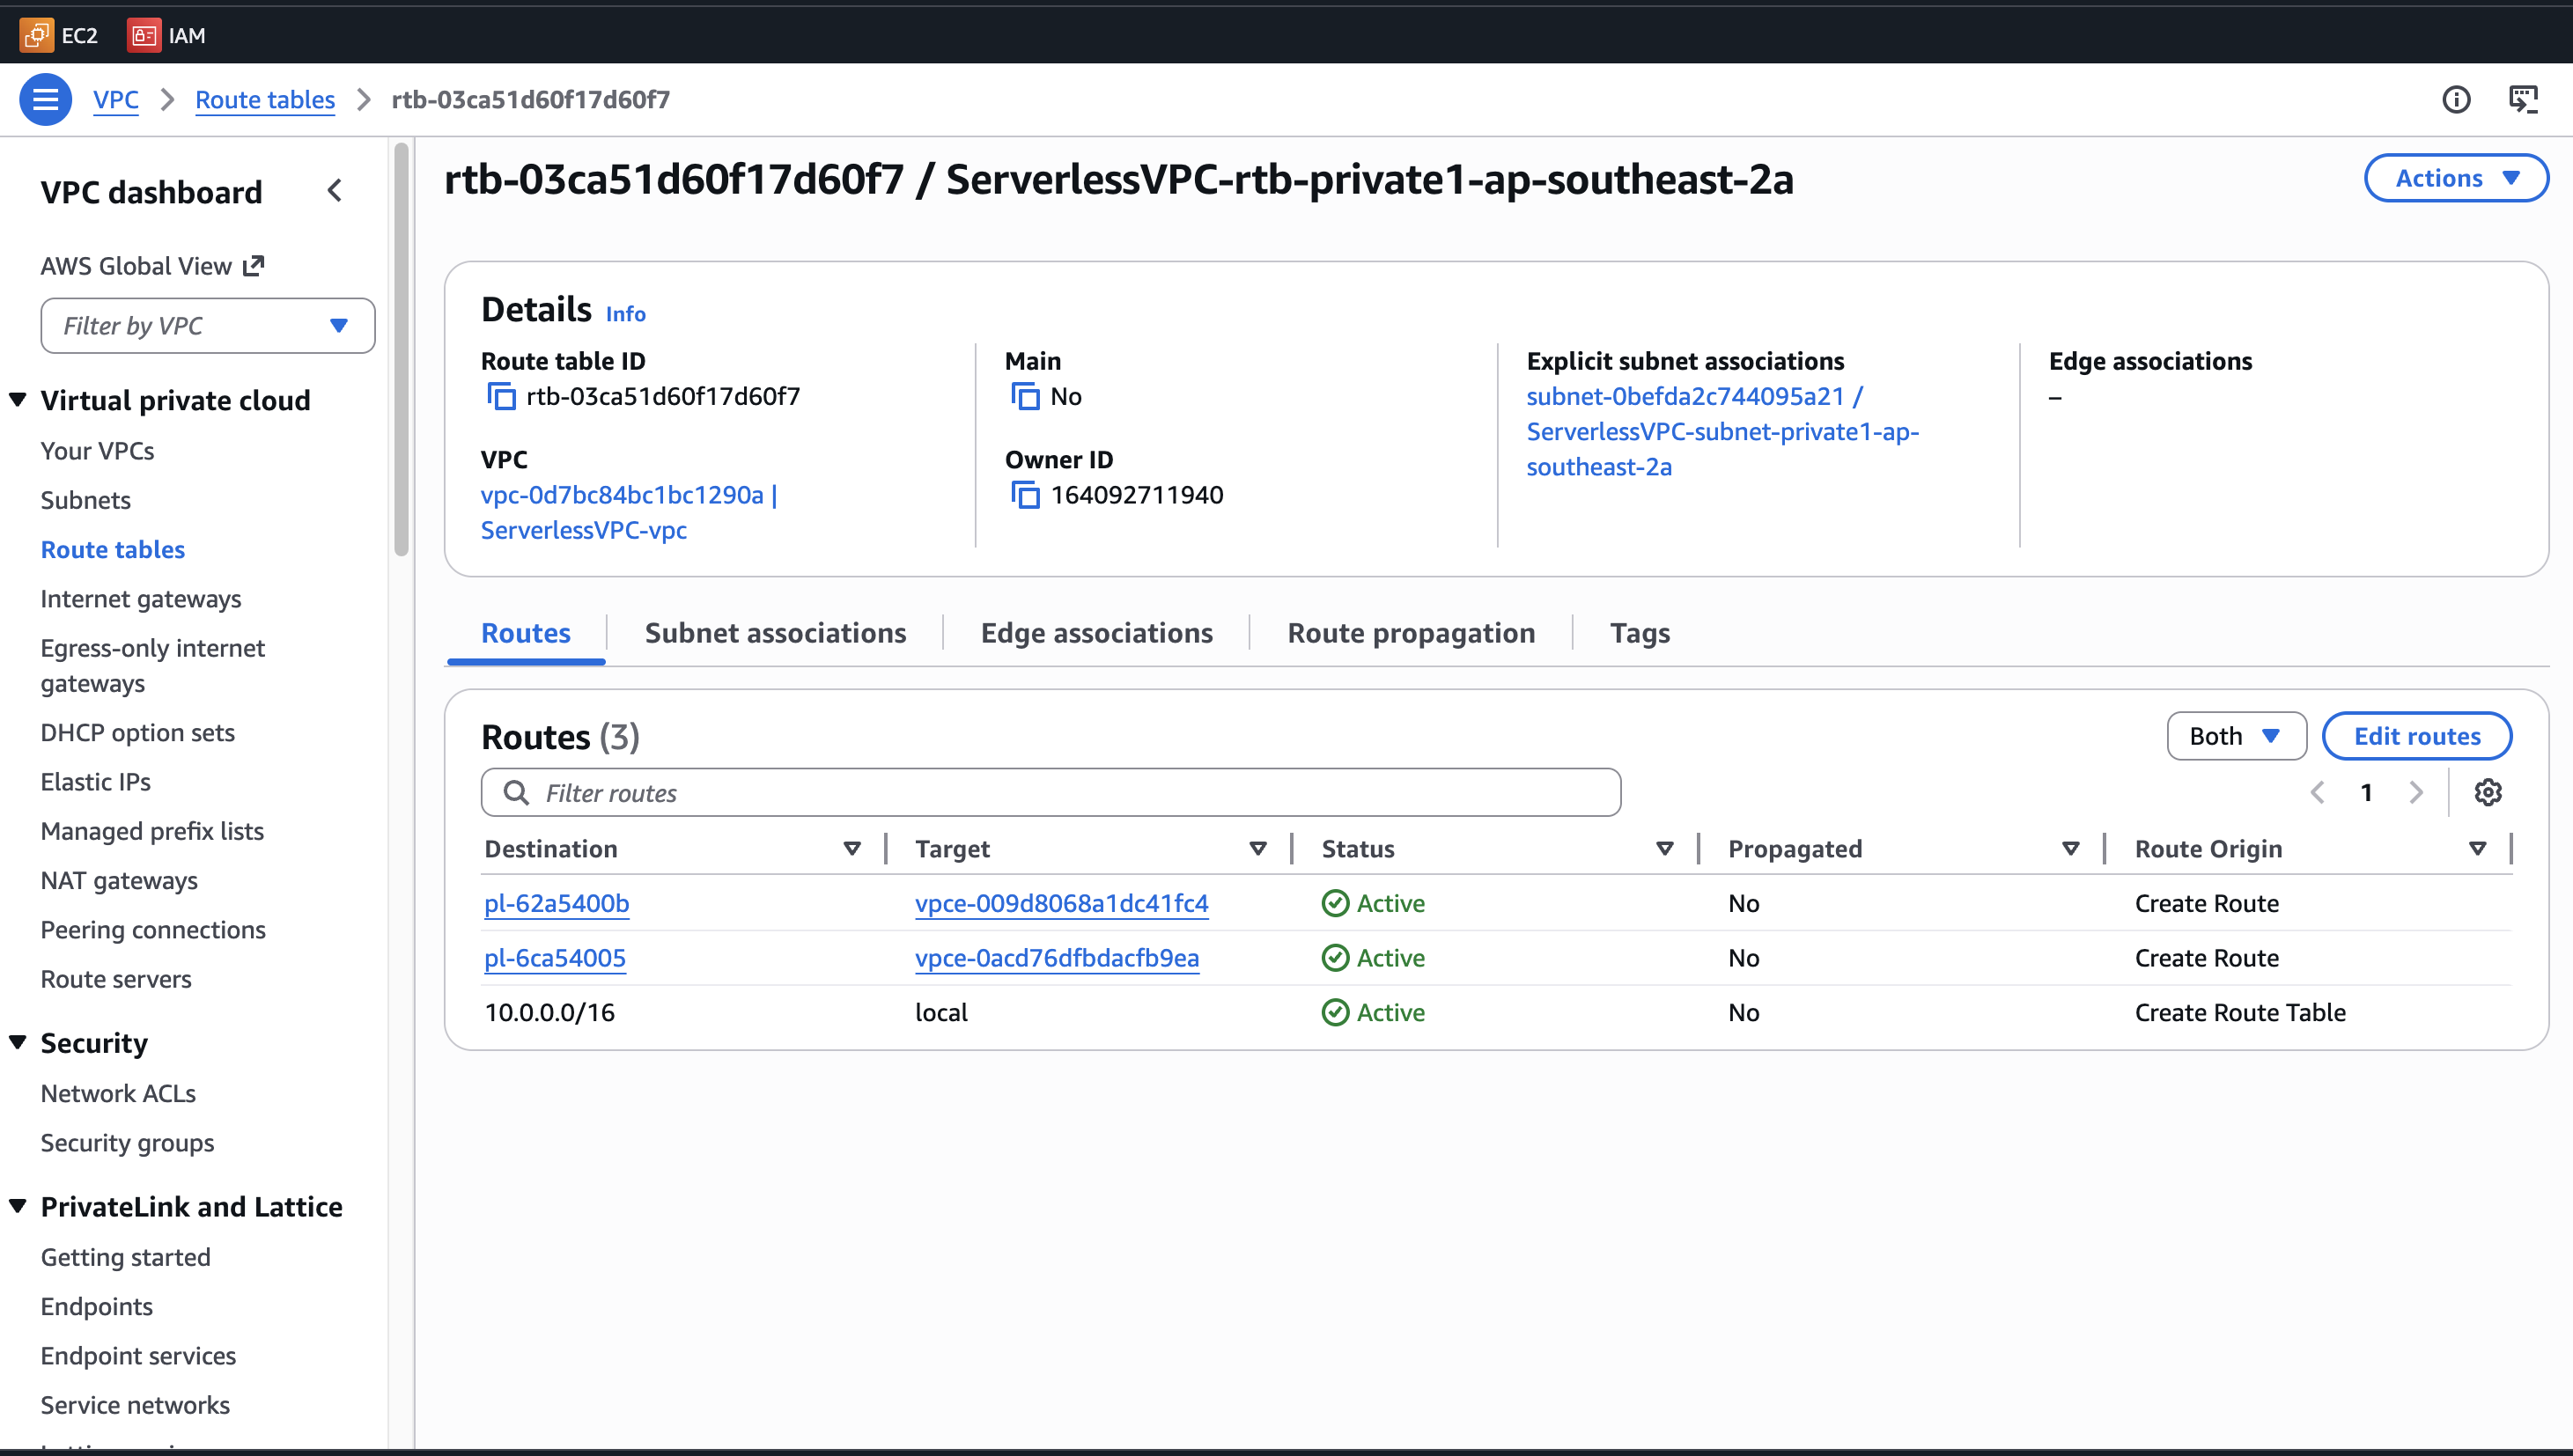
\includegraphics[width=0.9\textwidth]{img/NE-3_route_table.png}
\caption{Route Table với entry pl-xxxxx → vpce-xxxxx}
\label{fig:ne3}
\end{figure}

Route entries:
\begin{itemize}
    \item Destination: 10.0.0.0/16 → Target: local (VPC internal routing)
    \item Destination: pl-xxxxx (DynamoDB Prefix List) → Target: vpce-xxxxx (VPC Endpoint)
\end{itemize}

\subsubsection{NE-4: No NAT Gateway Exists}

Hình \ref{fig:ne4} xác nhận không có NAT Gateway nào tồn tại trong VPC. Điều này quan trọng để đảm bảo chi phí bằng 0 (NAT Gateway tốn ~\$32/month).

\begin{figure}[H]
\centering
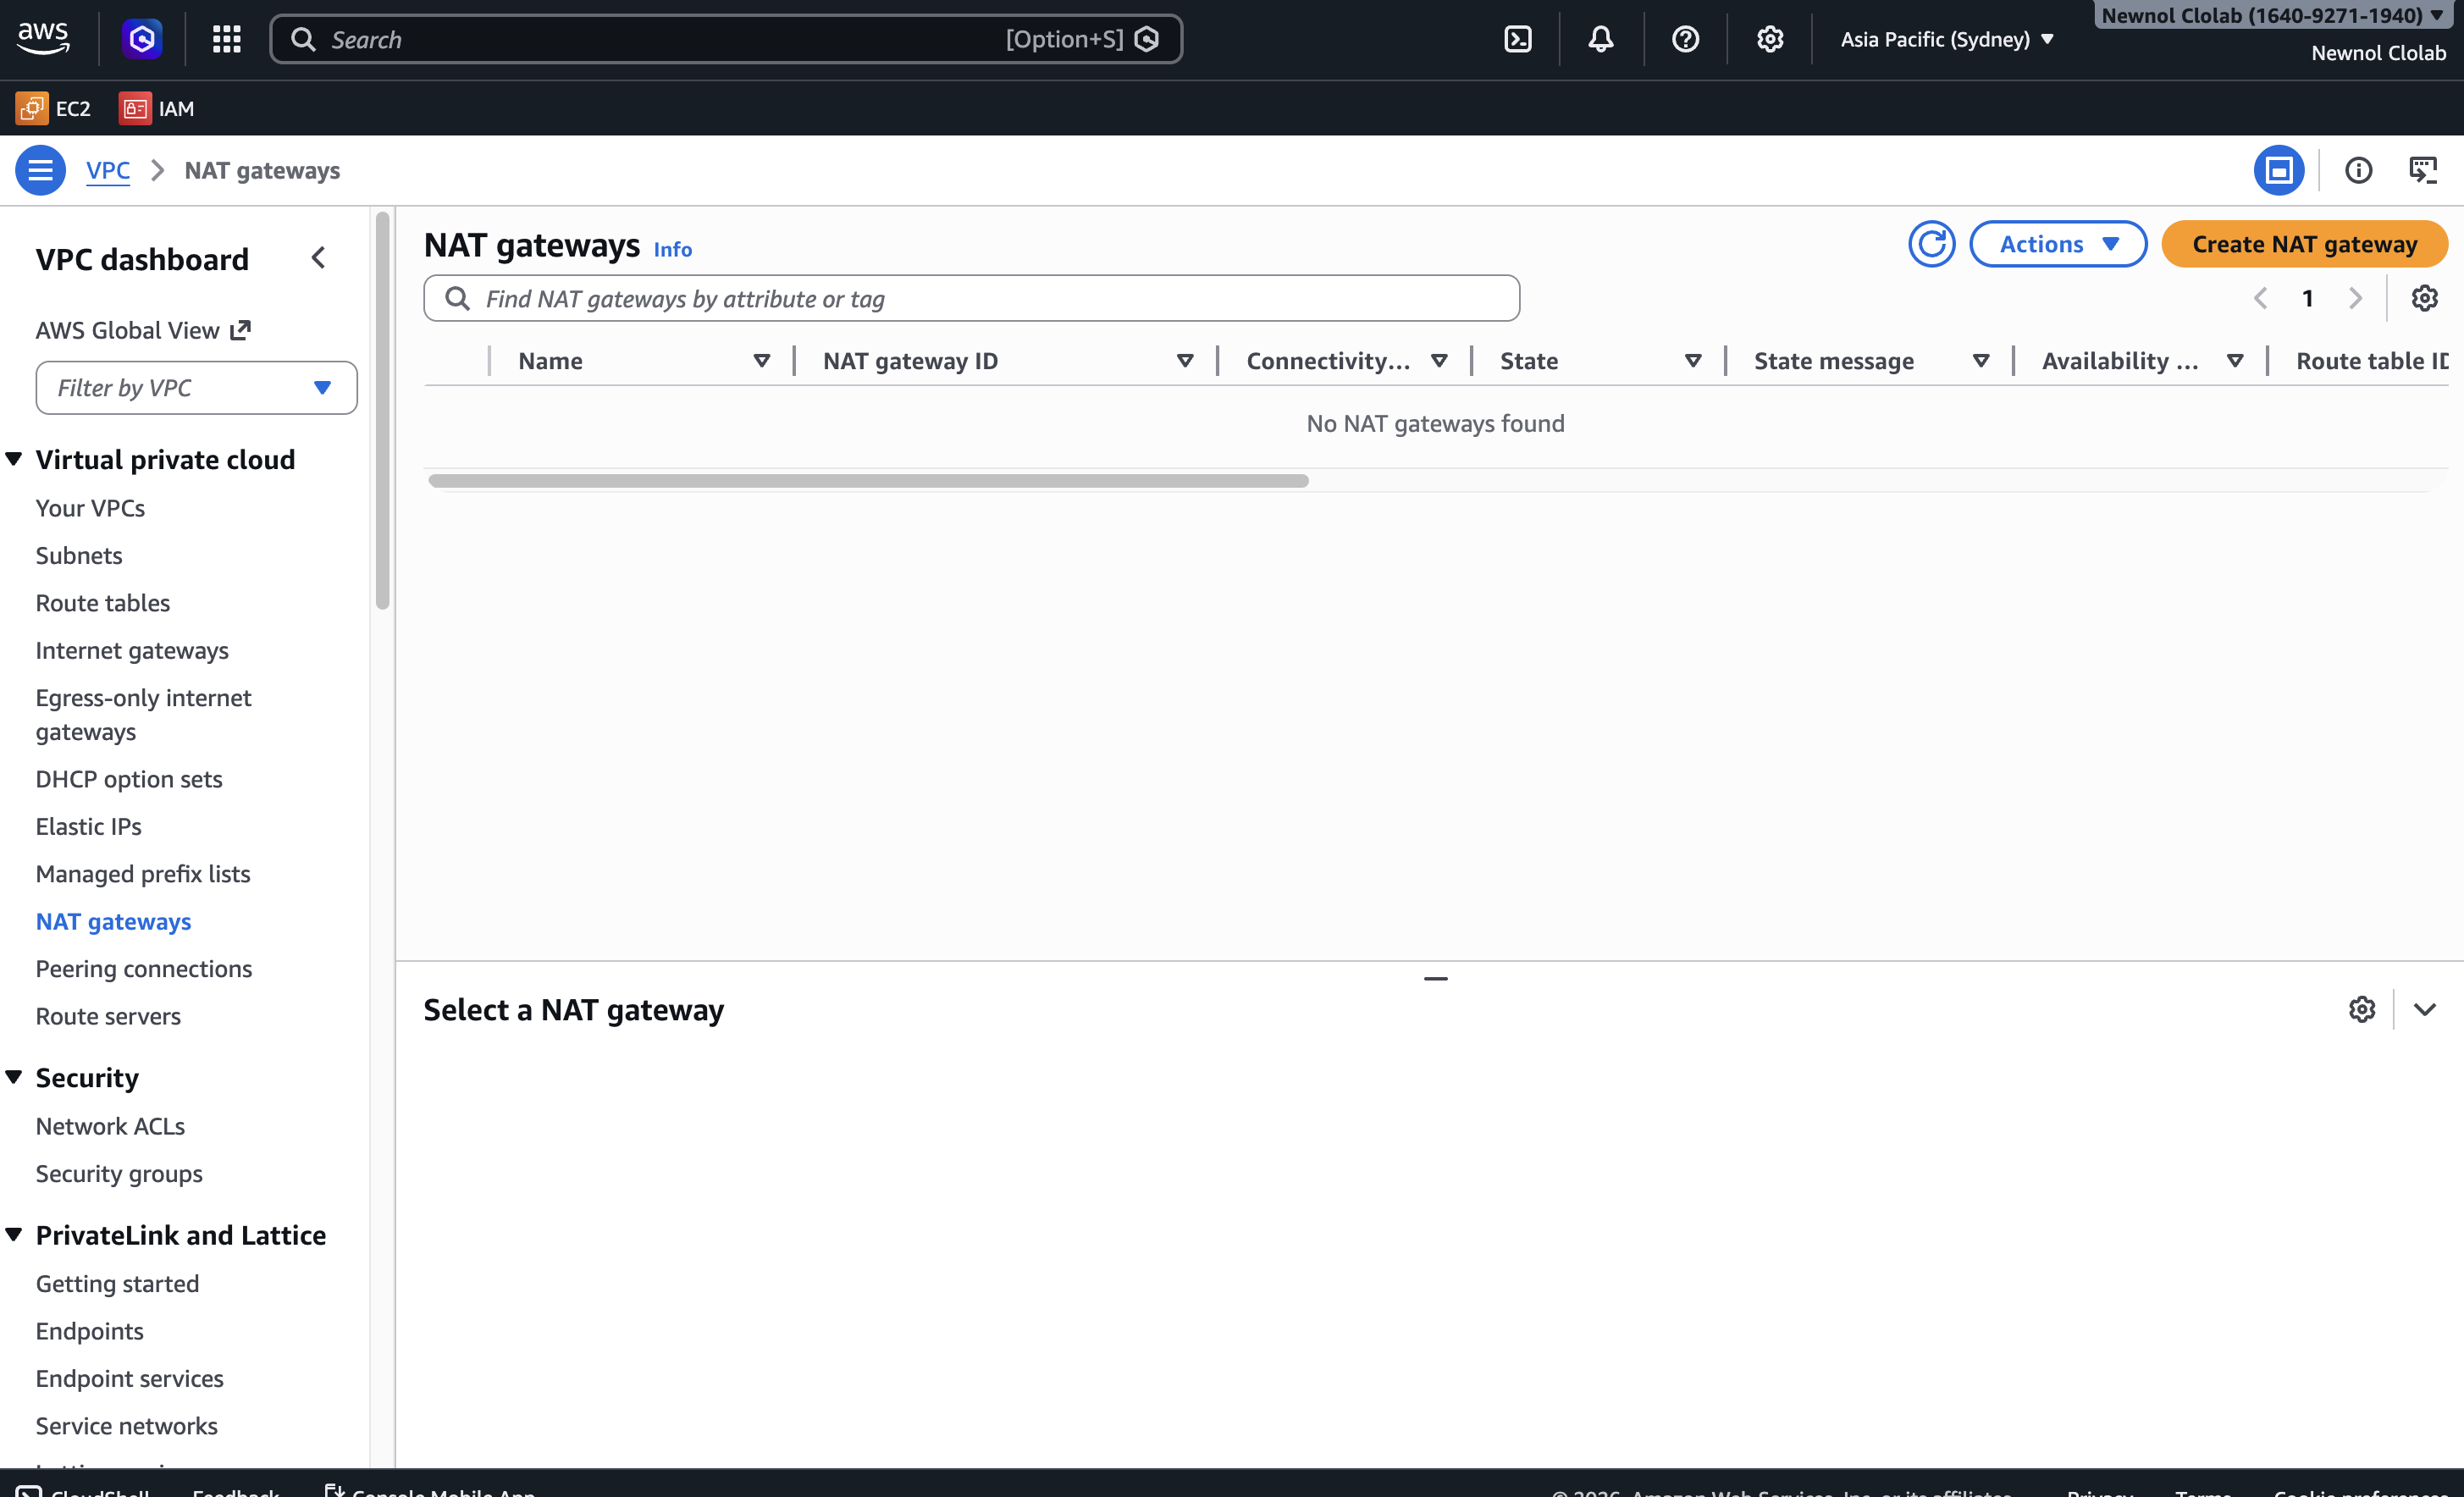
\includegraphics[width=0.9\textwidth]{img/NE-4_no_nat_gateway.png}
\caption{Danh sách NAT Gateways trống - không có NAT Gateway}
\label{fig:ne4}
\end{figure}

\subsubsection{NE-5: Lambda Successfully Calls DynamoDB}

Hình \ref{fig:ne5} cho thấy CloudWatch log của Lambda invocation thành công, với DynamoDB call trả về status code 200. Điều này chứng minh kết nối private qua VPC Endpoint hoạt động đúng.

\begin{figure}[H]
\centering
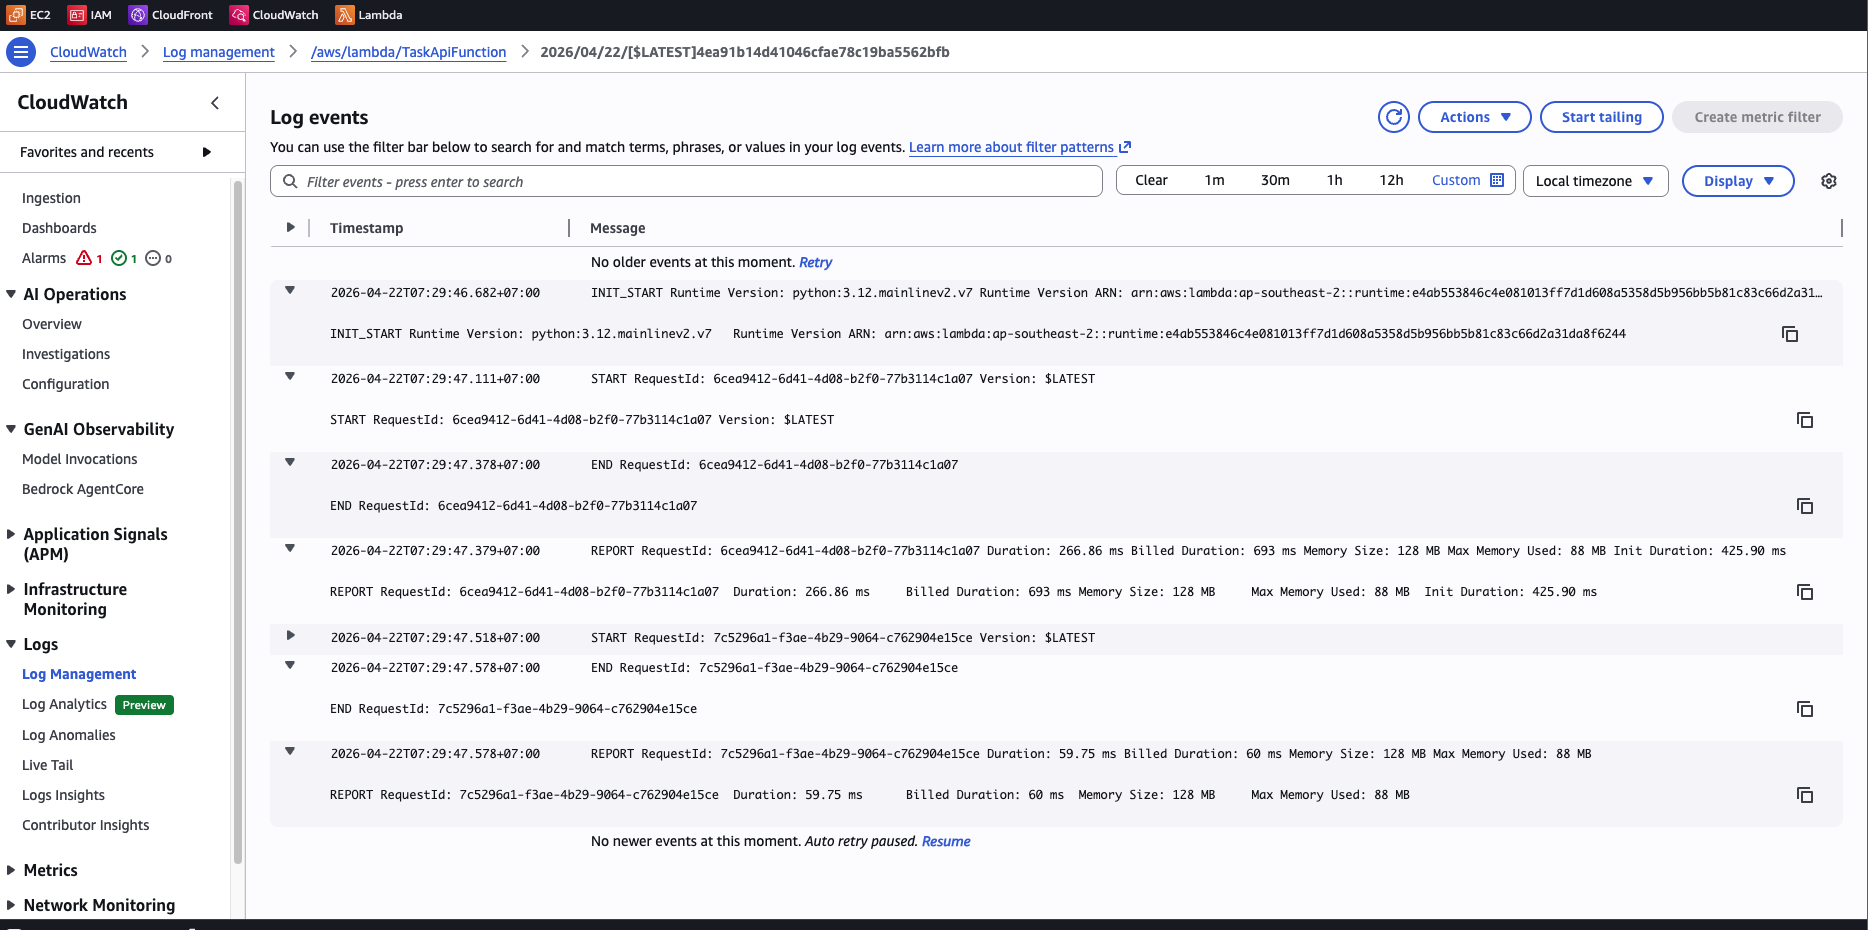
\includegraphics[width=0.9\textwidth]{img/NE-5.png}
\caption{CloudWatch log - Lambda gọi DynamoDB thành công qua VPC Endpoint}
\label{fig:ne5}
\end{figure}

Log details:
\begin{itemize}
    \item Request ID: xxxxx-xxxxx-xxxxx
    \item Duration: ~200ms
    \item Billed Duration: 300ms
    \item Memory Used: 128 MB
    \item DynamoDB response: StatusCode 200
    \item No NetworkingError hoặc UnauthorizedAccess error
\end{itemize}

\subsection{IAM Security Evidence}
\label{ssec:iam_security}

\subsubsection{IM-1: Two Separate IAM Roles}

Hình \ref{fig:im1} hiển thị hai IAM Roles riêng biệt đã được tạo cho các Lambda functions khác nhau, tuân thủ nguyên tắc Least Privilege.

\begin{figure}[H]
\centering
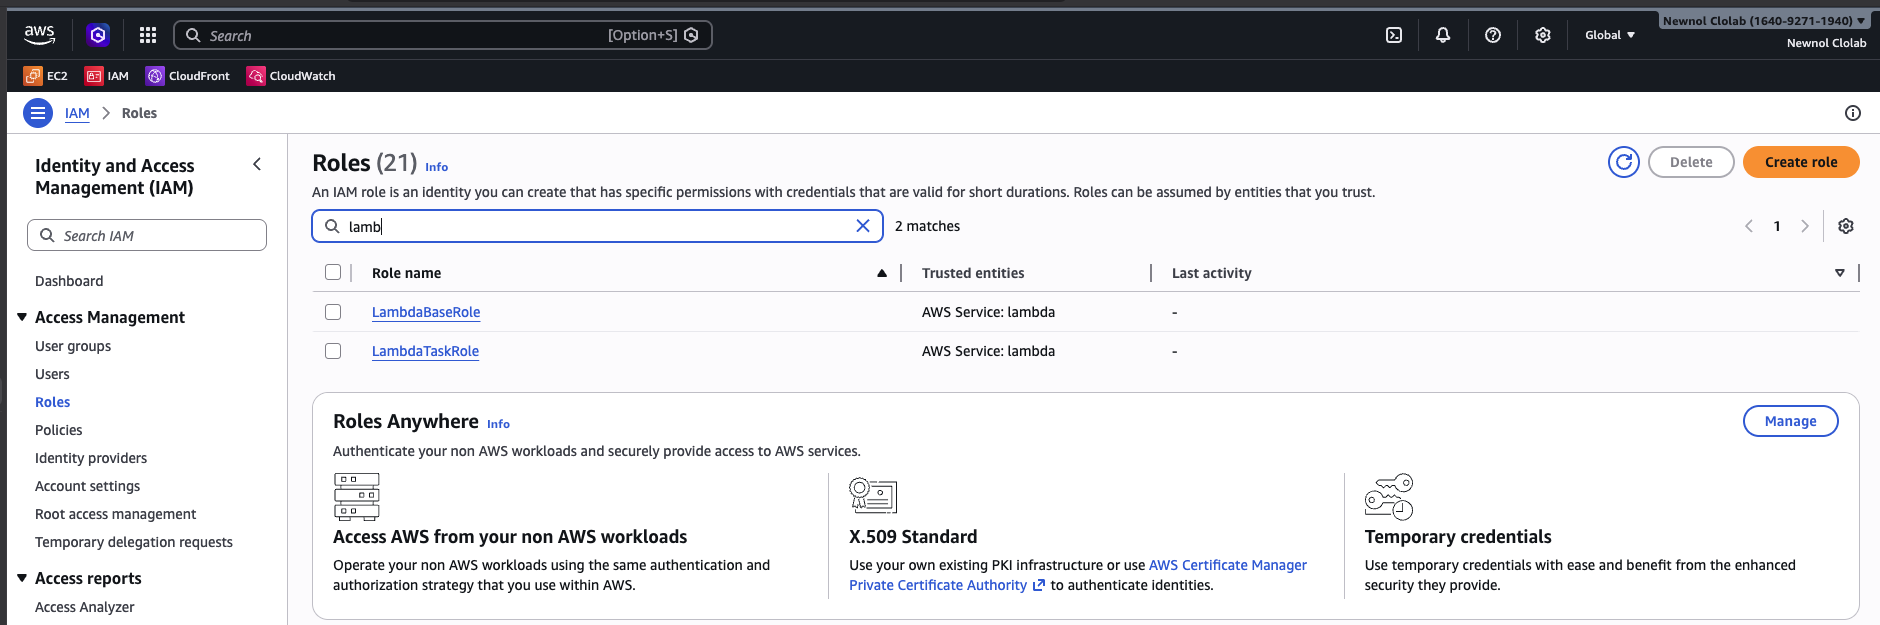
\includegraphics[width=0.9\textwidth]{img/IM-1_IAM_role.png}
\caption{Hai IAM Roles riêng biệt: LambdaTaskRole và LambdaBaseRole}
\label{fig:im1}
\end{figure}

Roles:
\begin{itemize}
    \item \textbf{LambdaTaskRole:} Cho Lambda xử lý tasks - có quyền DynamoDB + CloudWatch Logs + ENI
    \item \textbf{LambdaBaseRole:} Cho Lambda khác - chỉ có CloudWatch Logs + ENI
\end{itemize}

\subsubsection{IM-2: Policy Specifies Exact Resource ARN}

Hình \ref{fig:im2a} và \ref{fig:im2b} cho thấy IAM Policy JSON với Resource field chỉ định chính xác DynamoDB table ARN, không sử dụng wildcard (*).

\begin{figure}[H]
\centering
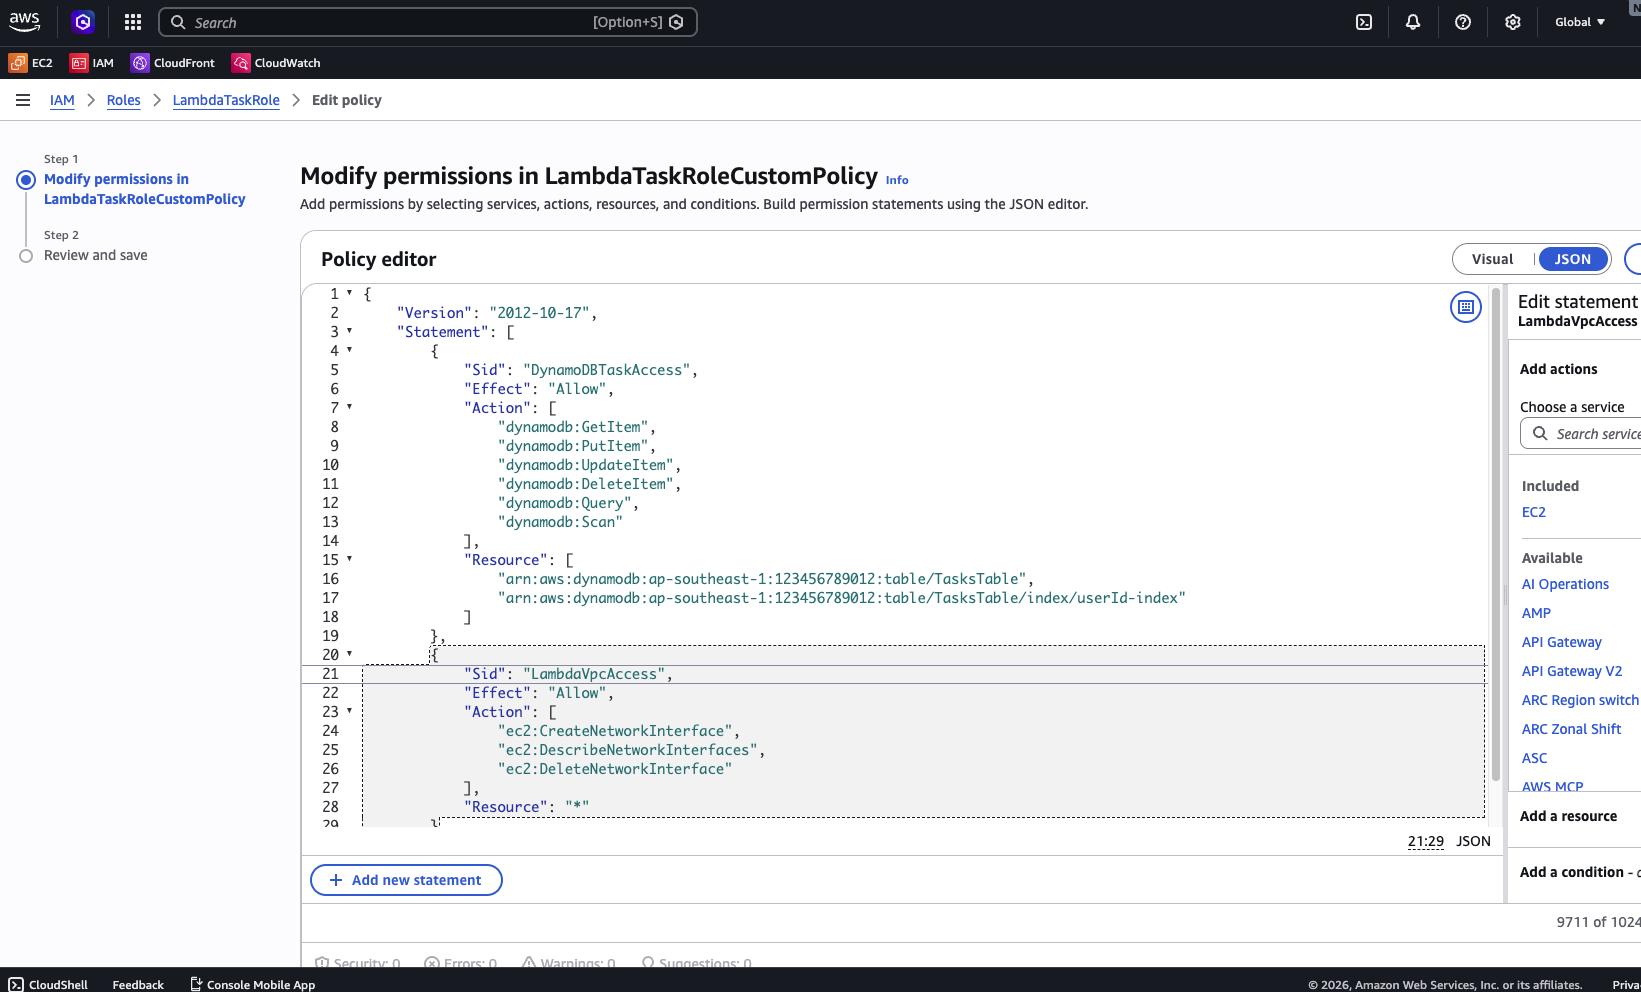
\includegraphics[width=0.9\textwidth]{img/IM-2_LambdaTaskRole.png}
\caption{LambdaTaskRole Policy với specific DynamoDB table ARN}
\label{fig:im2a}
\end{figure}

\begin{figure}[H]
\centering
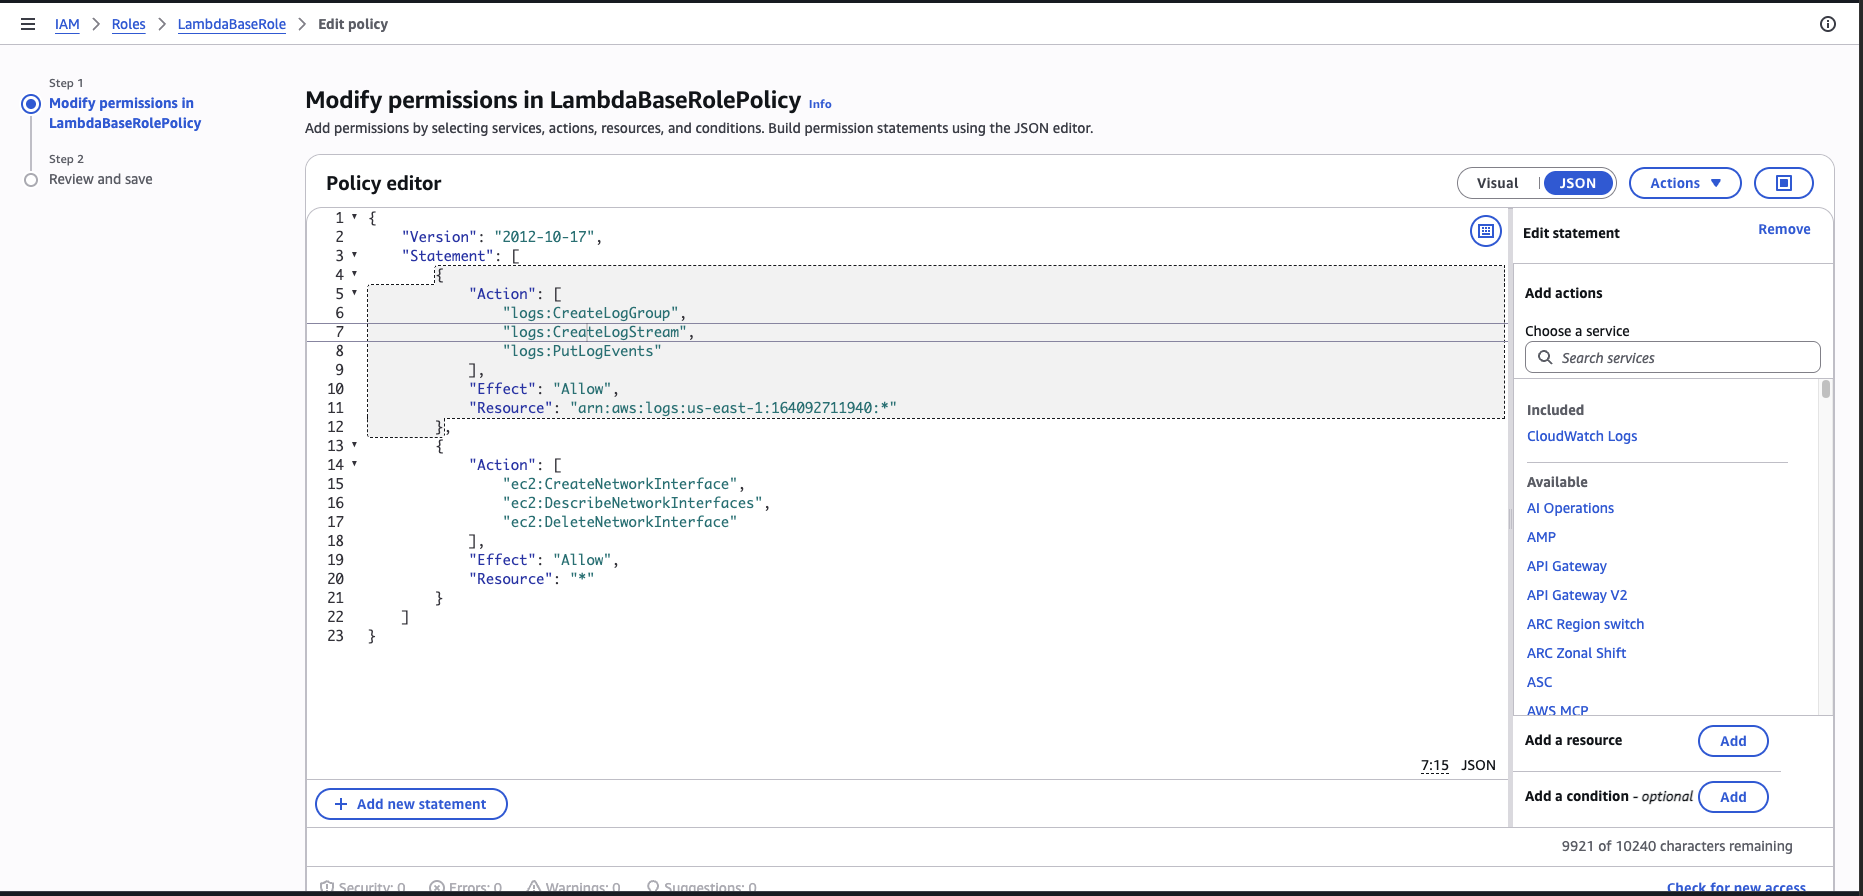
\includegraphics[width=0.9\textwidth]{img/IM-2_LambdaBaseRole.png}
\caption{LambdaBaseRole Policy - không có DynamoDB permissions}
\label{fig:im2b}
\end{figure}

Policy highlights:
\begin{itemize}
    \item Resource: "arn:aws:dynamodb:ap-southeast-1:123456789012:table/Tasks"
    \item Resource: "arn:aws:dynamodb:ap-southeast-1:123456789012:table/Tasks/index/*"
    \item Không có wildcard "*" cho DynamoDB resources
\end{itemize}

\subsubsection{IM-3: Lambda Attached to Correct Role}

Hình \ref{fig:im3} xác nhận Lambda function đã được attach đúng IAM Role với permissions phù hợp.

\begin{figure}[H]
\centering
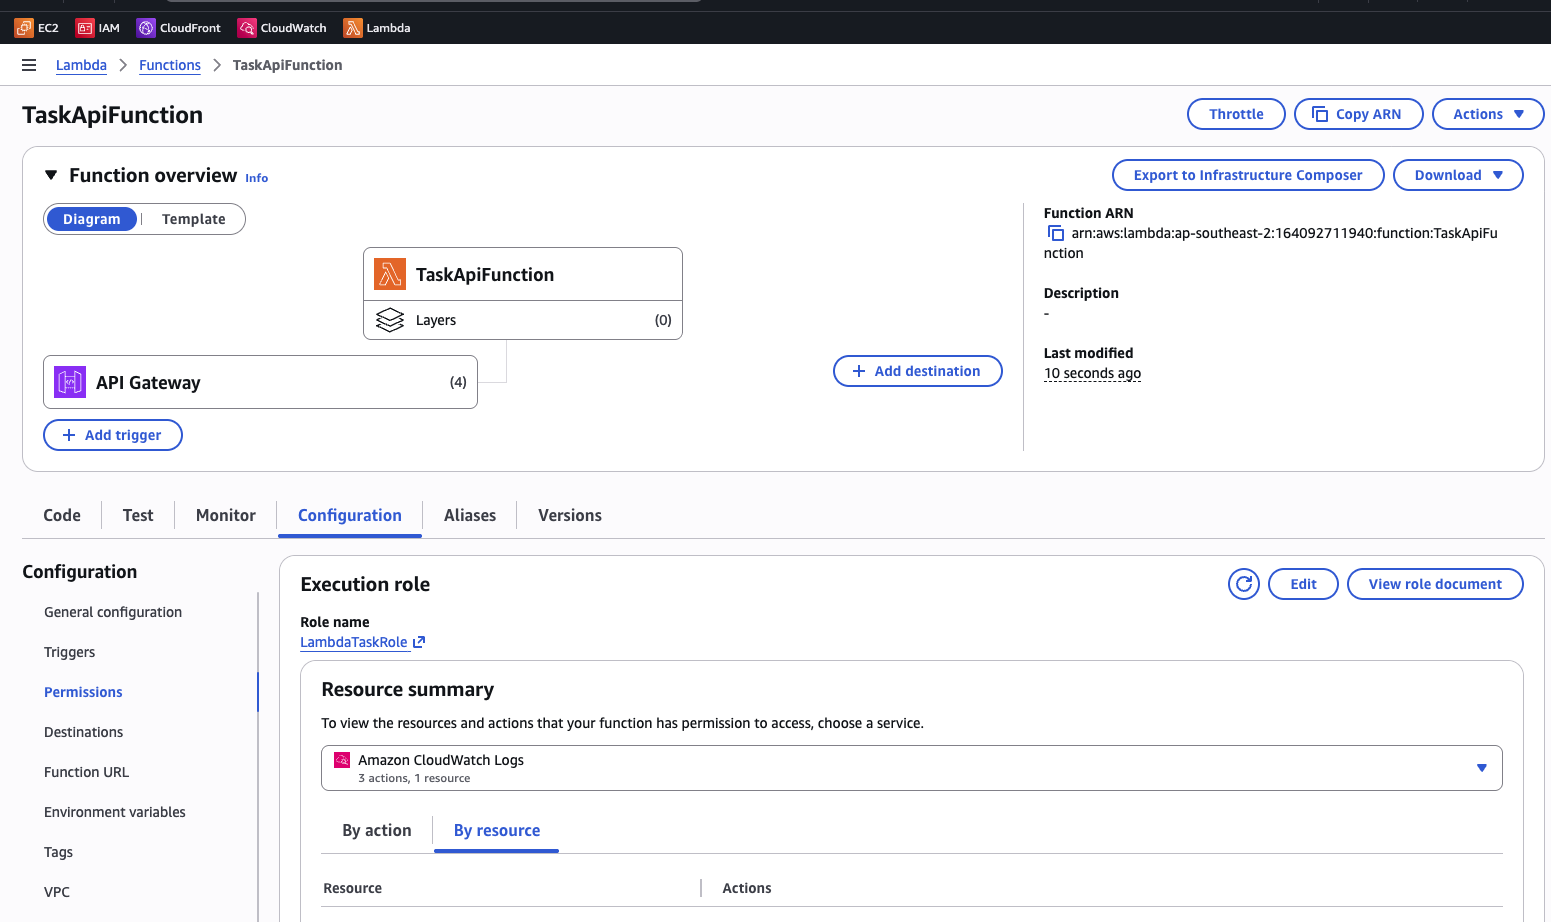
\includegraphics[width=0.9\textwidth]{img/IM-3_TaskApiFunction.png}
\caption{Lambda Configuration - Execution role: LambdaTaskRole}
\label{fig:im3}
\end{figure}

\subsection{Tổng kết bảo mật}
\label{ssec:security_summary}

Hệ thống đã triển khai đầy đủ các biện pháp bảo mật theo yêu cầu:

\begin{table}[H]
\centering
\begin{tabular}{|l|l|c|}
\hline
\textbf{ID} & \textbf{Evidence Item} & \textbf{Status} \\
\hline
SE-1 & S3 Block Public Access enabled & ✓ \\
SE-2 & Direct S3 access rejected (403) & ✓ \\
SE-3 & CloudFront access succeeds (200) & ✓ \\
SE-4 & OAC attached to CloudFront & ✓ \\
NE-1 & VPC Endpoint for DynamoDB & ✓ \\
NE-2 & Lambda VpcConfig attached & ✓ \\
NE-3 & Route Table has endpoint route & ✓ \\
NE-4 & No NAT Gateway exists & ✓ \\
NE-5 & Lambda calls DynamoDB successfully & ✓ \\
IM-1 & Two separate IAM Roles & ✓ \\
IM-2 & Policy with specific ARN & ✓ \\
IM-3 & Lambda attached to correct Role & ✓ \\
\hline
\end{tabular}
\caption{Checklist bằng chứng bảo mật}
\label{tab:security_checklist}
\end{table}
